%%%%%%%%%%%%%%%%%%%%%%%%%%%%%%%%%%%%%%%%%
% Masters/Doctoral Thesis 
% LaTeX Template
% Version 2.5 (27/8/17)
%
% This template was downloaded from:
% http://www.LaTeXTemplates.com
%
% Version 2.x major modifications by:
% Vel (vel@latextemplates.com)
%
% This template is based on a template by:
% Steve Gunn (http://users.ecs.soton.ac.uk/srg/softwaretools/document/templates/)
% Sunil Patel (http://www.sunilpatel.co.uk/thesis-template/)
%
% Template license:
% CC BY-NC-SA 3.0 (http://creativecommons.org/licenses/by-nc-sa/3.0/)
%
%%%%%%%%%%%%%%%%%%%%%%%%%%%%%%%%%%%%%%%%%

%----------------------------------------------------------------------------------------
%	PACKAGES AND OTHER DOCUMENT CONFIGURATIONS
%----------------------------------------------------------------------------------------

\documentclass[
11pt, % The default document font size, options: 10pt, 11pt, 12pt
%oneside, % Two side (alternating margins) for binding by default, uncomment to switch to one side
english, % ngerman for German
singlespacing, % Single line spacing, alternatives: onehalfspacing or doublespacing
%draft, % Uncomment to enable draft mode (no pictures, no links, overfull hboxes indicated)
%nolistspacing, % If the document is onehalfspacing or doublespacing, uncomment this to set spacing in lists to single
%liststotoc, % Uncomment to add the list of figures/tables/etc to the table of contents
%toctotoc, % Uncomment to add the main table of contents to the table of contents
%parskip, % Uncomment to add space between paragraphs
%nohyperref, % Uncomment to not load the hyperref package
headsepline, % Uncomment to get a line under the header
%chapterinoneline, % Uncomment to place the chapter title next to the number on one line
%consistentlayout, % Uncomment to change the layout of the declaration, abstract and acknowledgements pages to match the default layout
]{MastersDoctoralThesis} % The class file specifying the document structure

\usepackage[utf8]{inputenc} % Required for inputting international characters
\usepackage[T1]{fontenc} % Output font encoding for international characters

\usepackage{mathpazo} % Use the Palatino font by default

\usepackage[backend=bibtex,style=authoryear,natbib=true]{biblatex} % Use the bibtex backend with the authoryear citation style (which resembles APA)

\addbibresource{example.bib} % The filename of the bibliography

\usepackage[autostyle=true]{csquotes} % Required to generate language-dependent quotes in the bibliography

%----------------------------------------------------------------------------------------
%	MARGIN SETTINGS
%----------------------------------------------------------------------------------------

\geometry{
	paper=a4paper, % Change to letterpaper for US letter
	inner=2.5cm, % Inner margin
	outer=3.8cm, % Outer margin
	bindingoffset=.5cm, % Binding offset
	top=1.5cm, % Top margin
	bottom=1.5cm, % Bottom margin
	%showframe, % Uncomment to show how the type block is set on the page
}

%----------------------------------------------------------------------------------------
%	THESIS INFORMATION
%----------------------------------------------------------------------------------------

\thesistitle{Thesis Title} % Your thesis title, this is used in the title and abstract, print it elsewhere with \ttitle
\supervisor{Dr. James \textsc{Smith}} % Your supervisor's name, this is used in the title page, print it elsewhere with \supname
\examiner{} % Your examiner's name, this is not currently used anywhere in the template, print it elsewhere with \examname
\degree{Doctor of Philosophy} % Your degree name, this is used in the title page and abstract, print it elsewhere with \degreename
\author{John \textsc{Smith}} % Your name, this is used in the title page and abstract, print it elsewhere with \authorname
\addresses{} % Your address, this is not currently used anywhere in the template, print it elsewhere with \addressname

\subject{Biological Sciences} % Your subject area, this is not currently used anywhere in the template, print it elsewhere with \subjectname
\keywords{} % Keywords for your thesis, this is not currently used anywhere in the template, print it elsewhere with \keywordnames
\university{\href{http://www.university.com}{University Name}} % Your university's name and URL, this is used in the title page and abstract, print it elsewhere with \univname
\department{\href{http://department.university.com}{Department or School Name}} % Your department's name and URL, this is used in the title page and abstract, print it elsewhere with \deptname
\group{\href{http://researchgroup.university.com}{Research Group Name}} % Your research group's name and URL, this is used in the title page, print it elsewhere with \groupname
\faculty{\href{http://faculty.university.com}{Faculty Name}} % Your faculty's name and URL, this is used in the title page and abstract, print it elsewhere with \facname

\AtBeginDocument{
\hypersetup{pdftitle=\ttitle} % Set the PDF's title to your title
\hypersetup{pdfauthor=\authorname} % Set the PDF's author to your name
\hypersetup{pdfkeywords=\keywordnames} % Set the PDF's keywords to your keywords
}

\begin{document}

\frontmatter % Use roman page numbering style (i, ii, iii, iv...) for the pre-content pages

\pagestyle{plain} % Default to the plain heading style until the thesis style is called for the body content

%----------------------------------------------------------------------------------------
%	TITLE PAGE
%----------------------------------------------------------------------------------------

\begin{titlepage}
\begin{center}

\vspace*{.06\textheight}
{\scshape\LARGE \univname\par}\vspace{1.5cm} % University name
\textsc{\Large Doctoral Thesis}\\[0.5cm] % Thesis type

\HRule \\[0.4cm] % Horizontal line
{\huge \bfseries \ttitle\par}\vspace{0.4cm} % Thesis title
\HRule \\[1.5cm] % Horizontal line
 
\begin{minipage}[t]{0.4\textwidth}
\begin{flushleft} \large
\emph{Author:}\\
\href{http://www.johnsmith.com}{\authorname} % Author name - remove the \href bracket to remove the link
\end{flushleft}
\end{minipage}
\begin{minipage}[t]{0.4\textwidth}
\begin{flushright} \large
\emph{Supervisor:} \\
\href{http://www.jamessmith.com}{\supname} % Supervisor name - remove the \href bracket to remove the link  
\end{flushright}
\end{minipage}\\[3cm]
 
\vfill

\large \textit{A thesis submitted in fulfillment of the requirements\\ for the degree of \degreename}\\[0.3cm] % University requirement text
\textit{in the}\\[0.4cm]
\groupname\\\deptname\\[2cm] % Research group name and department name
 
\vfill

{\large \today}\\[4cm] % Date
%\includegraphics{Logo} % University/department logo - uncomment to place it
 
\vfill
\end{center}
\end{titlepage}

%----------------------------------------------------------------------------------------
%	DECLARATION PAGE
%----------------------------------------------------------------------------------------

\begin{declaration}
\addchaptertocentry{\authorshipname} % Add the declaration to the table of contents
\noindent I, \authorname, declare that this thesis titled, \enquote{\ttitle} and the work presented in it are my own. I confirm that:

\begin{itemize} 
\item This work was done wholly or mainly while in candidature for a research degree at this University.
\item Where any part of this thesis has previously been submitted for a degree or any other qualification at this University or any other institution, this has been clearly stated.
\item Where I have consulted the published work of others, this is always clearly attributed.
\item Where I have quoted from the work of others, the source is always given. With the exception of such quotations, this thesis is entirely my own work.
\item I have acknowledged all main sources of help.
\item Where the thesis is based on work done by myself jointly with others, I have made clear exactly what was done by others and what I have contributed myself.\\
\end{itemize}
 
\noindent Signed:\\
\rule[0.5em]{25em}{0.5pt} % This prints a line for the signature
 
\noindent Date:\\
\rule[0.5em]{25em}{0.5pt} % This prints a line to write the date
\end{declaration}

\cleardoublepage

%----------------------------------------------------------------------------------------
%	QUOTATION PAGE
%----------------------------------------------------------------------------------------

\vspace*{0.2\textheight}

\noindent\enquote{\itshape Thanks to my solid academic training, today I can write hundreds of words on virtually any topic without possessing a shred of information, which is how I got a good job in journalism.}\bigbreak

\hfill Dave Barry

%----------------------------------------------------------------------------------------
%	ABSTRACT PAGE
%----------------------------------------------------------------------------------------

\begin{abstract}
\addchaptertocentry{\abstractname} % Add the abstract to the table of contents
The Thesis Abstract is written here (and usually kept to just this page). The page is kept centered vertically so can expand into the blank space above the title too\ldots
\end{abstract}

%----------------------------------------------------------------------------------------
%	ACKNOWLEDGEMENTS
%----------------------------------------------------------------------------------------

\begin{acknowledgements}
\addchaptertocentry{\acknowledgementname} % Add the acknowledgements to the table of contents
The acknowledgments and the people to thank go here, don't forget to include your project advisor\ldots
\end{acknowledgements}

%----------------------------------------------------------------------------------------
%	LIST OF CONTENTS/FIGURES/TABLES PAGES
%----------------------------------------------------------------------------------------

\tableofcontents % Prints the main table of contents

\listoffigures % Prints the list of figures

\listoftables % Prints the list of tables

%----------------------------------------------------------------------------------------
%	ABBREVIATIONS
%----------------------------------------------------------------------------------------

\begin{abbreviations}{ll} % Include a list of abbreviations (a table of two columns)

\textbf{LAH} & \textbf{L}ist \textbf{A}bbreviations \textbf{H}ere\\
\textbf{WSF} & \textbf{W}hat (it) \textbf{S}tands \textbf{F}or\\

\end{abbreviations}

%----------------------------------------------------------------------------------------
%	PHYSICAL CONSTANTS/OTHER DEFINITIONS
%----------------------------------------------------------------------------------------

\begin{constants}{lr@{${}={}$}l} % The list of physical constants is a three column table

% The \SI{}{} command is provided by the siunitx package, see its documentation for instructions on how to use it

Speed of Light & $c_{0}$ & \SI{2.99792458e8}{\meter\per\second} (exact)\\
%Constant Name & $Symbol$ & $Constant Value$ with units\\

\end{constants}

%----------------------------------------------------------------------------------------
%	SYMBOLS
%----------------------------------------------------------------------------------------

\begin{symbols}{lll} % Include a list of Symbols (a three column table)

$a$ & distance & \si{\meter} \\
$P$ & power & \si{\watt} (\si{\joule\per\second}) \\
%Symbol & Name & Unit \\

\addlinespace % Gap to separate the Roman symbols from the Greek

$\omega$ & angular frequency & \si{\radian} \\

\end{symbols}

%----------------------------------------------------------------------------------------
%	DEDICATION
%----------------------------------------------------------------------------------------

\dedicatory{For/Dedicated to/To my\ldots} 

%----------------------------------------------------------------------------------------
%	THESIS CONTENT - CHAPTERS
%----------------------------------------------------------------------------------------

\mainmatter % Begin numeric (1,2,3...) page numbering

\pagestyle{thesis} % Return the page headers back to the "thesis" style

% Include the chapters of the thesis as separate files from the Chapters folder
% Uncomment the lines as you write the chapters

% Chapter 1

\chapter{Chapter Title Here} % Main chapter title

\label{Chapter1} % For referencing the chapter elsewhere, use \ref{Chapter1} 

%----------------------------------------------------------------------------------------

% Define some commands to keep the formatting separated from the content 
\newcommand{\keyword}[1]{\textbf{#1}}
\newcommand{\tabhead}[1]{\textbf{#1}}
\newcommand{\code}[1]{\texttt{#1}}
\newcommand{\file}[1]{\texttt{\bfseries#1}}
\newcommand{\option}[1]{\texttt{\itshape#1}}

%----------------------------------------------------------------------------------------

\section{Welcome and Thank You}
Welcome to this \LaTeX{} Thesis Template, a beautiful and easy to use template for writing a thesis using the \LaTeX{} typesetting system.

If you are writing a thesis (or will be in the future) and its subject is technical or mathematical (though it doesn't have to be), then creating it in \LaTeX{} is highly recommended as a way to make sure you can just get down to the essential writing without having to worry over formatting or wasting time arguing with your word processor.

\LaTeX{} is easily able to professionally typeset documents that run to hundreds or thousands of pages long. With simple mark-up commands, it automatically sets out the table of contents, margins, page headers and footers and keeps the formatting consistent and beautiful. One of its main strengths is the way it can easily typeset mathematics, even \emph{heavy} mathematics. Even if those equations are the most horribly twisted and most difficult mathematical problems that can only be solved on a super-computer, you can at least count on \LaTeX{} to make them look stunning.

%----------------------------------------------------------------------------------------

\section{Learning \LaTeX{}}

\LaTeX{} is not a \textsc{wysiwyg} (What You See is What You Get) program, unlike word processors such as Microsoft Word or Apple's Pages. Instead, a document written for \LaTeX{} is actually a simple, plain text file that contains \emph{no formatting}. You tell \LaTeX{} how you want the formatting in the finished document by writing in simple commands amongst the text, for example, if I want to use \emph{italic text for emphasis}, I write the \verb|\emph{text}| command and put the text I want in italics in between the curly braces. This means that \LaTeX{} is a \enquote{mark-up} language, very much like HTML.

\subsection{A (not so short) Introduction to \LaTeX{}}

If you are new to \LaTeX{}, there is a very good eBook -- freely available online as a PDF file -- called, \enquote{The Not So Short Introduction to \LaTeX{}}. The book's title is typically shortened to just \emph{lshort}. You can download the latest version (as it is occasionally updated) from here:
\url{http://www.ctan.org/tex-archive/info/lshort/english/lshort.pdf}

It is also available in several other languages. Find yours from the list on this page: \url{http://www.ctan.org/tex-archive/info/lshort/}

It is recommended to take a little time out to learn how to use \LaTeX{} by creating several, small `test' documents, or having a close look at several templates on:\\ 
\url{http://www.LaTeXTemplates.com}\\ 
Making the effort now means you're not stuck learning the system when what you \emph{really} need to be doing is writing your thesis.

\subsection{A Short Math Guide for \LaTeX{}}

If you are writing a technical or mathematical thesis, then you may want to read the document by the AMS (American Mathematical Society) called, \enquote{A Short Math Guide for \LaTeX{}}. It can be found online here:
\url{http://www.ams.org/tex/amslatex.html}
under the \enquote{Additional Documentation} section towards the bottom of the page.

\subsection{Common \LaTeX{} Math Symbols}
There are a multitude of mathematical symbols available for \LaTeX{} and it would take a great effort to learn the commands for them all. The most common ones you are likely to use are shown on this page:
\url{http://www.sunilpatel.co.uk/latex-type/latex-math-symbols/}

You can use this page as a reference or crib sheet, the symbols are rendered as large, high quality images so you can quickly find the \LaTeX{} command for the symbol you need.

\subsection{\LaTeX{} on a Mac}
 
The \LaTeX{} distribution is available for many systems including Windows, Linux and Mac OS X. The package for OS X is called MacTeX and it contains all the applications you need -- bundled together and pre-customized -- for a fully working \LaTeX{} environment and work flow.
 
MacTeX includes a custom dedicated \LaTeX{} editor called TeXShop for writing your `\file{.tex}' files and BibDesk: a program to manage your references and create your bibliography section just as easily as managing songs and creating playlists in iTunes.

%----------------------------------------------------------------------------------------

\section{Getting Started with this Template}

If you are familiar with \LaTeX{}, then you should explore the directory structure of the template and then proceed to place your own information into the \emph{THESIS INFORMATION} block of the \file{main.tex} file. You can then modify the rest of this file to your unique specifications based on your degree/university. Section \ref{FillingFile} on page \pageref{FillingFile} will help you do this. Make sure you also read section \ref{ThesisConventions} about thesis conventions to get the most out of this template.

If you are new to \LaTeX{} it is recommended that you carry on reading through the rest of the information in this document.

Before you begin using this template you should ensure that its style complies with the thesis style guidelines imposed by your institution. In most cases this template style and layout will be suitable. If it is not, it may only require a small change to bring the template in line with your institution's recommendations. These modifications will need to be done on the \file{MastersDoctoralThesis.cls} file.

\subsection{About this Template}

This \LaTeX{} Thesis Template is originally based and created around a \LaTeX{} style file created by Steve R.\ Gunn from the University of Southampton (UK), department of Electronics and Computer Science. You can find his original thesis style file at his site, here:
\url{http://www.ecs.soton.ac.uk/~srg/softwaretools/document/templates/}

Steve's \file{ecsthesis.cls} was then taken by Sunil Patel who modified it by creating a skeleton framework and folder structure to place the thesis files in. The resulting template can be found on Sunil's site here:
\url{http://www.sunilpatel.co.uk/thesis-template}

Sunil's template was made available through \url{http://www.LaTeXTemplates.com} where it was modified many times based on user requests and questions. Version 2.0 and onwards of this template represents a major modification to Sunil's template and is, in fact, hardly recognisable. The work to make version 2.0 possible was carried out by \href{mailto:vel@latextemplates.com}{Vel} and Johannes Böttcher.

%----------------------------------------------------------------------------------------

\section{What this Template Includes}

\subsection{Folders}

This template comes as a single zip file that expands out to several files and folders. The folder names are mostly self-explanatory:

\keyword{Appendices} -- this is the folder where you put the appendices. Each appendix should go into its own separate \file{.tex} file. An example and template are included in the directory.

\keyword{Chapters} -- this is the folder where you put the thesis chapters. A thesis usually has about six chapters, though there is no hard rule on this. Each chapter should go in its own separate \file{.tex} file and they can be split as:
\begin{itemize}
\item Chapter 1: Introduction to the thesis topic
\item Chapter 2: Background information and theory
\item Chapter 3: (Laboratory) experimental setup
\item Chapter 4: Details of experiment 1
\item Chapter 5: Details of experiment 2
\item Chapter 6: Discussion of the experimental results
\item Chapter 7: Conclusion and future directions
\end{itemize}
This chapter layout is specialised for the experimental sciences, your discipline may be different.

\keyword{Figures} -- this folder contains all figures for the thesis. These are the final images that will go into the thesis document.

\subsection{Files}

Included are also several files, most of them are plain text and you can see their contents in a text editor. After initial compilation, you will see that more auxiliary files are created by \LaTeX{} or BibTeX and which you don't need to delete or worry about:

\keyword{example.bib} -- this is an important file that contains all the bibliographic information and references that you will be citing in the thesis for use with BibTeX. You can write it manually, but there are reference manager programs available that will create and manage it for you. Bibliographies in \LaTeX{} are a large subject and you may need to read about BibTeX before starting with this. Many modern reference managers will allow you to export your references in BibTeX format which greatly eases the amount of work you have to do.

\keyword{MastersDoctoralThesis.cls} -- this is an important file. It is the class file that tells \LaTeX{} how to format the thesis. 

\keyword{main.pdf} -- this is your beautifully typeset thesis (in the PDF file format) created by \LaTeX{}. It is supplied in the PDF with the template and after you compile the template you should get an identical version.

\keyword{main.tex} -- this is an important file. This is the file that you tell \LaTeX{} to compile to produce your thesis as a PDF file. It contains the framework and constructs that tell \LaTeX{} how to layout the thesis. It is heavily commented so you can read exactly what each line of code does and why it is there. After you put your own information into the \emph{THESIS INFORMATION} block -- you have now started your thesis!

Files that are \emph{not} included, but are created by \LaTeX{} as auxiliary files include:

\keyword{main.aux} -- this is an auxiliary file generated by \LaTeX{}, if it is deleted \LaTeX{} simply regenerates it when you run the main \file{.tex} file.

\keyword{main.bbl} -- this is an auxiliary file generated by BibTeX, if it is deleted, BibTeX simply regenerates it when you run the \file{main.aux} file. Whereas the \file{.bib} file contains all the references you have, this \file{.bbl} file contains the references you have actually cited in the thesis and is used to build the bibliography section of the thesis.

\keyword{main.blg} -- this is an auxiliary file generated by BibTeX, if it is deleted BibTeX simply regenerates it when you run the main \file{.aux} file.

\keyword{main.lof} -- this is an auxiliary file generated by \LaTeX{}, if it is deleted \LaTeX{} simply regenerates it when you run the main \file{.tex} file. It tells \LaTeX{} how to build the \emph{List of Figures} section.

\keyword{main.log} -- this is an auxiliary file generated by \LaTeX{}, if it is deleted \LaTeX{} simply regenerates it when you run the main \file{.tex} file. It contains messages from \LaTeX{}, if you receive errors and warnings from \LaTeX{}, they will be in this \file{.log} file.

\keyword{main.lot} -- this is an auxiliary file generated by \LaTeX{}, if it is deleted \LaTeX{} simply regenerates it when you run the main \file{.tex} file. It tells \LaTeX{} how to build the \emph{List of Tables} section.

\keyword{main.out} -- this is an auxiliary file generated by \LaTeX{}, if it is deleted \LaTeX{} simply regenerates it when you run the main \file{.tex} file.

So from this long list, only the files with the \file{.bib}, \file{.cls} and \file{.tex} extensions are the most important ones. The other auxiliary files can be ignored or deleted as \LaTeX{} and BibTeX will regenerate them.

%----------------------------------------------------------------------------------------

\section{Filling in Your Information in the \file{main.tex} File}\label{FillingFile}

You will need to personalise the thesis template and make it your own by filling in your own information. This is done by editing the \file{main.tex} file in a text editor or your favourite LaTeX environment.

Open the file and scroll down to the third large block titled \emph{THESIS INFORMATION} where you can see the entries for \emph{University Name}, \emph{Department Name}, etc \ldots

Fill out the information about yourself, your group and institution. You can also insert web links, if you do, make sure you use the full URL, including the \code{http://} for this. If you don't want these to be linked, simply remove the \verb|\href{url}{name}| and only leave the name.

When you have done this, save the file and recompile \code{main.tex}. All the information you filled in should now be in the PDF, complete with web links. You can now begin your thesis proper!

%----------------------------------------------------------------------------------------

\section{The \code{main.tex} File Explained}

The \file{main.tex} file contains the structure of the thesis. There are plenty of written comments that explain what pages, sections and formatting the \LaTeX{} code is creating. Each major document element is divided into commented blocks with titles in all capitals to make it obvious what the following bit of code is doing. Initially there seems to be a lot of \LaTeX{} code, but this is all formatting, and it has all been taken care of so you don't have to do it.

Begin by checking that your information on the title page is correct. For the thesis declaration, your institution may insist on something different than the text given. If this is the case, just replace what you see with what is required in the \emph{DECLARATION PAGE} block.

Then comes a page which contains a funny quote. You can put your own, or quote your favourite scientist, author, person, and so on. Make sure to put the name of the person who you took the quote from.

Following this is the abstract page which summarises your work in a condensed way and can almost be used as a standalone document to describe what you have done. The text you write will cause the heading to move up so don't worry about running out of space.

Next come the acknowledgements. On this page, write about all the people who you wish to thank (not forgetting parents, partners and your advisor/supervisor).

The contents pages, list of figures and tables are all taken care of for you and do not need to be manually created or edited. The next set of pages are more likely to be optional and can be deleted since they are for a more technical thesis: insert a list of abbreviations you have used in the thesis, then a list of the physical constants and numbers you refer to and finally, a list of mathematical symbols used in any formulae. Making the effort to fill these tables means the reader has a one-stop place to refer to instead of searching the internet and references to try and find out what you meant by certain abbreviations or symbols.

The list of symbols is split into the Roman and Greek alphabets. Whereas the abbreviations and symbols ought to be listed in alphabetical order (and this is \emph{not} done automatically for you) the list of physical constants should be grouped into similar themes.

The next page contains a one line dedication. Who will you dedicate your thesis to?

Finally, there is the block where the chapters are included. Uncomment the lines (delete the \code{\%} character) as you write the chapters. Each chapter should be written in its own file and put into the \emph{Chapters} folder and named \file{Chapter1}, \file{Chapter2}, etc\ldots Similarly for the appendices, uncomment the lines as you need them. Each appendix should go into its own file and placed in the \emph{Appendices} folder.

After the preamble, chapters and appendices finally comes the bibliography. The bibliography style (called \option{authoryear}) is used for the bibliography and is a fully featured style that will even include links to where the referenced paper can be found online. Do not underestimate how grateful your reader will be to find that a reference to a paper is just a click away. Of course, this relies on you putting the URL information into the BibTeX file in the first place.

%----------------------------------------------------------------------------------------

\section{Thesis Features and Conventions}\label{ThesisConventions}

To get the best out of this template, there are a few conventions that you may want to follow.

One of the most important (and most difficult) things to keep track of in such a long document as a thesis is consistency. Using certain conventions and ways of doing things (such as using a Todo list) makes the job easier. Of course, all of these are optional and you can adopt your own method.

\subsection{Printing Format}

This thesis template is designed for double sided printing (i.e. content on the front and back of pages) as most theses are printed and bound this way. Switching to one sided printing is as simple as uncommenting the \option{oneside} option of the \code{documentclass} command at the top of the \file{main.tex} file. You may then wish to adjust the margins to suit specifications from your institution.

The headers for the pages contain the page number on the outer side (so it is easy to flick through to the page you want) and the chapter name on the inner side.

The text is set to 11 point by default with single line spacing, again, you can tune the text size and spacing should you want or need to using the options at the very start of \file{main.tex}. The spacing can be changed similarly by replacing the \option{singlespacing} with \option{onehalfspacing} or \option{doublespacing}.

\subsection{Using US Letter Paper}

The paper size used in the template is A4, which is the standard size in Europe. If you are using this thesis template elsewhere and particularly in the United States, then you may have to change the A4 paper size to the US Letter size. This can be done in the margins settings section in \file{main.tex}.

Due to the differences in the paper size, the resulting margins may be different to what you like or require (as it is common for institutions to dictate certain margin sizes). If this is the case, then the margin sizes can be tweaked by modifying the values in the same block as where you set the paper size. Now your document should be set up for US Letter paper size with suitable margins.

\subsection{References}

The \code{biblatex} package is used to format the bibliography and inserts references such as this one \parencite{Reference1}. The options used in the \file{main.tex} file mean that the in-text citations of references are formatted with the author(s) listed with the date of the publication. Multiple references are separated by semicolons (e.g. \parencite{Reference2, Reference1}) and references with more than three authors only show the first author with \emph{et al.} indicating there are more authors (e.g. \parencite{Reference3}). This is done automatically for you. To see how you use references, have a look at the \file{Chapter1.tex} source file. Many reference managers allow you to simply drag the reference into the document as you type.

Scientific references should come \emph{before} the punctuation mark if there is one (such as a comma or period). The same goes for footnotes\footnote{Such as this footnote, here down at the bottom of the page.}. You can change this but the most important thing is to keep the convention consistent throughout the thesis. Footnotes themselves should be full, descriptive sentences (beginning with a capital letter and ending with a full stop). The APA6 states: \enquote{Footnote numbers should be superscripted, [...], following any punctuation mark except a dash.} The Chicago manual of style states: \enquote{A note number should be placed at the end of a sentence or clause. The number follows any punctuation mark except the dash, which it precedes. It follows a closing parenthesis.}

The bibliography is typeset with references listed in alphabetical order by the first author's last name. This is similar to the APA referencing style. To see how \LaTeX{} typesets the bibliography, have a look at the very end of this document (or just click on the reference number links in in-text citations).

\subsubsection{A Note on bibtex}

The bibtex backend used in the template by default does not correctly handle unicode character encoding (i.e. "international" characters). You may see a warning about this in the compilation log and, if your references contain unicode characters, they may not show up correctly or at all. The solution to this is to use the biber backend instead of the outdated bibtex backend. This is done by finding this in \file{main.tex}: \option{backend=bibtex} and changing it to \option{backend=biber}. You will then need to delete all auxiliary BibTeX files and navigate to the template directory in your terminal (command prompt). Once there, simply type \code{biber main} and biber will compile your bibliography. You can then compile \file{main.tex} as normal and your bibliography will be updated. An alternative is to set up your LaTeX editor to compile with biber instead of bibtex, see \href{http://tex.stackexchange.com/questions/154751/biblatex-with-biber-configuring-my-editor-to-avoid-undefined-citations/}{here} for how to do this for various editors.

\subsection{Tables}

Tables are an important way of displaying your results, below is an example table which was generated with this code:

{\small
\begin{verbatim}
\begin{table}
\caption{The effects of treatments X and Y on the four groups studied.}
\label{tab:treatments}
\centering
\begin{tabular}{l l l}
\toprule
\tabhead{Groups} & \tabhead{Treatment X} & \tabhead{Treatment Y} \\
\midrule
1 & 0.2 & 0.8\\
2 & 0.17 & 0.7\\
3 & 0.24 & 0.75\\
4 & 0.68 & 0.3\\
\bottomrule\\
\end{tabular}
\end{table}
\end{verbatim}
}

\begin{table}
\caption{The effects of treatments X and Y on the four groups studied.}
\label{tab:treatments}
\centering
\begin{tabular}{l l l}
\toprule
\tabhead{Groups} & \tabhead{Treatment X} & \tabhead{Treatment Y} \\
\midrule
1 & 0.2 & 0.8\\
2 & 0.17 & 0.7\\
3 & 0.24 & 0.75\\
4 & 0.68 & 0.3\\
\bottomrule\\
\end{tabular}
\end{table}

You can reference tables with \verb|\ref{<label>}| where the label is defined within the table environment. See \file{Chapter1.tex} for an example of the label and citation (e.g. Table~\ref{tab:treatments}).

\subsection{Figures}

There will hopefully be many figures in your thesis (that should be placed in the \emph{Figures} folder). The way to insert figures into your thesis is to use a code template like this:
\begin{verbatim}
\begin{figure}
\centering

\includegraphics{Figures/Electron}
\decoRule
\caption[An Electron]{An electron (artist's impression).}
\label{fig:Electron}
\end{figure}
\end{verbatim}
Also look in the source file. Putting this code into the source file produces the picture of the electron that you can see in the figure below.

\begin{figure}[th]
\centering

\includegraphics{Figures/Electron}
\decoRule
\caption[An Electron]{An electron (artist's impression).}
\label{fig:Electron}
\end{figure}

Sometimes figures don't always appear where you write them in the source. The placement depends on how much space there is on the page for the figure. Sometimes there is not enough room to fit a figure directly where it should go (in relation to the text) and so \LaTeX{} puts it at the top of the next page. Positioning figures is the job of \LaTeX{} and so you should only worry about making them look good!

Figures usually should have captions just in case you need to refer to them (such as in Figure~\ref{fig:Electron}). The \verb|\caption| command contains two parts, the first part, inside the square brackets is the title that will appear in the \emph{List of Figures}, and so should be short. The second part in the curly brackets should contain the longer and more descriptive caption text.

The \verb|\decoRule| command is optional and simply puts an aesthetic horizontal line below the image. If you do this for one image, do it for all of them.

\LaTeX{} is capable of using images in pdf, jpg and png format.

\subsection{Typesetting mathematics}

If your thesis is going to contain heavy mathematical content, be sure that \LaTeX{} will make it look beautiful, even though it won't be able to solve the equations for you.

The \enquote{Not So Short Introduction to \LaTeX} (available on \href{http://www.ctan.org/tex-archive/info/lshort/english/lshort.pdf}{CTAN}) should tell you everything you need to know for most cases of typesetting mathematics. If you need more information, a much more thorough mathematical guide is available from the AMS called, \enquote{A Short Math Guide to \LaTeX} and can be downloaded from:
\url{ftp://ftp.ams.org/pub/tex/doc/amsmath/short-math-guide.pdf}

There are many different \LaTeX{} symbols to remember, luckily you can find the most common symbols in \href{http://ctan.org/pkg/comprehensive}{The Comprehensive \LaTeX~Symbol List}.

You can write an equation, which is automatically given an equation number by \LaTeX{} like this:
\begin{verbatim}
\begin{equation}
E = mc^{2}
\label{eqn:Einstein}
\end{equation}
\end{verbatim}

This will produce Einstein's famous energy-matter equivalence equation:
\begin{equation}
E = mc^{2}
\label{eqn:Einstein}
\end{equation}

All equations you write (which are not in the middle of paragraph text) are automatically given equation numbers by \LaTeX{}. If you don't want a particular equation numbered, use the unnumbered form:
\begin{verbatim}
\[ a^{2}=4 \]
\end{verbatim}

%----------------------------------------------------------------------------------------

\section{Sectioning and Subsectioning}

You should break your thesis up into nice, bite-sized sections and subsections. \LaTeX{} automatically builds a table of Contents by looking at all the \verb|\chapter{}|, \verb|\section{}|  and \verb|\subsection{}| commands you write in the source.

The Table of Contents should only list the sections to three (3) levels. A \verb|chapter{}| is level zero (0). A \verb|\section{}| is level one (1) and so a \verb|\subsection{}| is level two (2). In your thesis it is likely that you will even use a \verb|subsubsection{}|, which is level three (3). The depth to which the Table of Contents is formatted is set within \file{MastersDoctoralThesis.cls}. If you need this changed, you can do it in \file{main.tex}.

%----------------------------------------------------------------------------------------

\section{In Closing}

You have reached the end of this mini-guide. You can now rename or overwrite this pdf file and begin writing your own \file{Chapter1.tex} and the rest of your thesis. The easy work of setting up the structure and framework has been taken care of for you. It's now your job to fill it out!

Good luck and have lots of fun!

\begin{flushright}
Guide written by ---\\
Sunil Patel: \href{http://www.sunilpatel.co.uk}{www.sunilpatel.co.uk}\\
Vel: \href{http://www.LaTeXTemplates.com}{LaTeXTemplates.com}
\end{flushright}

%%What is dominance in social psychology
%Nonverbal Behavior and the Vertical Dimension of Social Relations: A Meta-Analysis
%
%\textbf{several representation of dominance :} 
%For example, dominance can be defined as a personality trait involving the motive to control others, the self-
%perception of oneself as controlling others, and/or as a behavioral
%outcome (success in controlling others or their resources). Status,
%involving an ascribed or achieved quality implying respect and
%privilege, does not necessarily include the ability to control others
%or their resources.
%
% Similarly, power defined as the capacity or
%structurally sanctioned right to control others or their resources
%does not necessarily imply prestige or respect. Other distinctions
%have also been drawn, including different functional bases of
%power, such as reward power, expert power, referent power, or
%coercive power (French and Raven, 1959), and outcome dependency
%(Stevens  Fiske, 2000). Some writers conceptualize dominance
%in terms of social skill (e.g., Burgoon  Dunbar, 2000; Byrne,
%2001). Some writers define dominance as the enactment of certain
%nonverbal or verbal behaviors (Rosa  Mazur, 1979). Authors do
%not use the various verticality terms such as power, dominance,
%and status in consistent ways, and often the terms are used without
%a clear definition.
%
%\textbf{Burgoon and dunber 2010}
%

%
%
%La dominance, d'un autre côté, se réfère à des comportements interactionnels dépendant du contexte et de la relation, dans lesquels le pouvoir est rendu saillant et l'influence est atteinte %(Burgoon et al., 1998; Mack, 1974; Rogers-Millar & Millar, 1979)
%dans le contexte de l'échange interpersonnel, la dominance est basée sur une combinaison de tempérament individuel et de caractéristiques situationnelles qui encouragent un comportement dominant. 
%Le dominance interpersonnelle est un comportement de communication basé sur la relation qui dépend du contexte et des motivations des individus impliqués
%
 
%Comme l'ont noté Emerson (1962) et d'autres théoriciens, le pouvoir équivaut à dépendre des autres et suppose donc une relation sociale.
%
%\textbf{Dyadic power theory:}
%
%
%Elle se base sur les échanges sociaux de pouvoir sur 4 éléments
%
%\begin{enumerate}
%	\item cette définition s'étend pour prendre en compte les échanges sociaux qui inclut les stratégies de communications qui deviennent manifestes durant l'interaction
%	\item Contrôle relationnel : elle reconnaît que l'autorité d'utiliser ou d'échanger des ressources dans les interactions est souvent accordée aux individus par les normes sociétales ainsi que par l'histoire relationnelle propre aux individus impliqués dans l'interaction.
%	
%	\item Cette représentation insiste sur l'idée que le pouvoir doit être vu relativement, ou par rapport aux autres. Ainsi, il reconnaît que le pouvoir est une construction dynamique et multidimensionnelle qui incorpore les perspectives des deux individus dans l'interaction.
%	\item En cohérence avec une perspective de communication, il place l'interaction elle-même au centre des préoccupations. Les tentatives de prendre le contrôle de toute interaction donnée par la dominance, bien que déterminées par le pouvoir, sont au centre de la théorie car elles déterminent le résultat du processus  (la décision finale qui a des ramifications pour l'avenir de la relation).
%%\end{enumerate}
%
%
%
%
%\textbf{Interpersonal dominance paper}
%En préface, notre intention n'est pas de représenter les trois comme des perspectives exhaustives ou mutuellement exclusives sur la construction de la domination-soumission, mais plutôt de mettre en lumière les nombreuses facettes de cette dimension fondamentale des relations humaines.


\subsection{Trait de personnalité}
%Les chercheurs qui se sont intéressés à l'étude de la personnalité tendent à voir la personnalité comme stable \cite{burgoon2006nonverbal} et par conséquent, cherchent a définir des indicateurs de dominance stable permettant de de former  des profils comportementaux stables. 

La dominance comme trait de personnalité a connu une évolution où la littérature en psychologie a élargit le concept de la dominance au-delà des comportements d'agressivité.
En effet, les travaux en Éthologie et psychologie évolutive ont d'abord étudié la dominance comme un trait de personnalité innée qui confère à la personne la capacité d'exercer son pouvoir et sa domination, susciter la déférence et l'acquiescement, ou apaiser et se soumettre à un comportement conspécifique plus fort \cite{keltner1995signs,burgoon2006nonverbal}. Cependant, les travaux en Éthologie contemporaine s'éloignent de cette définition en faveur d'études pour la compréhension de l'interaction entre les organismes et leur environnement social \cite{burgoon2006nonverbal}.

Pour les psychologues de la personnalité, la dominance est considérée comme un trait individuel durable qui désigne le tempérament de la personne et les prédispositions comportementales de chacun \cite{cattell1970handbook,ridgeway1987nonverbal} tels que l'agression, l'ambition, l'argumentation,
assertivité, vantardise, confiance et détermination.
Les adjectifs communs utilisés pour décrire la personne dominante sont affirmés, agressifs, compétitifs, exigeant, égoïste et têtu. Plus précisément, la dominance en tant que variable de personnalité «montre un ajustement réaliste constant au succès et à l'échec de l'individu, à la santé ou à la maladie, aux capacités ou handicaps et aux forces extérieures relatives» \cite{cattell1970handbook,burgoon1998nature}.
En effet, selon  Emmons et McAdams \cite{emmons1991personal}, les individus avec un motif de haut pouvoir sont décrits comme voulant contrôler et influencer les autres, désirant la célébrité ou l'attention du public, et ayant la capacité de susciter l'émotion chez les autres. Dans la même veine, \cite{jackson1974personality} décrivent une personne dominante comme une personne qui cherche et maintient un rôle de leader dans un groupe. Ces personnes prennent en charge et guident les membres du groupe vers la réalisation d'objectifs louables à travers des tactiques d'influence, des manœuvres de contrôle de l'environnement et l'expression énergique de l'opinion \cite{burgoon1998nature}. 
A l'opposé, les individus non dominants ou soumis sont présentés comme coopératifs, modestes et obéissants, mais aussi obséquieux, doux, faibles, peu sûrs et évitant les situations qui nécessitent une affirmation de soi \cite{burgoon1998nature}. 

%Les habiletés sociales font partie de cette équation, car la capacité d'être énergique, de prendre des initiatives et d'être expressif mais détendu et équilibré \cite{burgoon2006nonverbal}. 
Par ailleurs, la dominance et soumission sont généralement révélés à travers le style de communication \cite{burgoon1998nature}. Une personne dominante va avoir plus d'assurance dans sa manière de communiquer, à être plus confiante, enthousiaste, énergique, active, compétitive, sûre d'elle, vaniteuse et direct. Ceci transparaît dans les comportements verbaux et non verbaux utilisés. Une personne dominante va  utiliser plus d'espace, avec un temps de conversation plus long et être capable d'avoir plus d'interruption réussies \cite{burgoon1998nature}. 

En revanche, une personne soumise va utiliser un mouvement contraint, une utilisation limitée de l'espace, de grandes quantités de regard tout en écoutant  \cite{burgoon1998nature}. Ces comportements sont présentés plus en détails dans la section ... 


\subsection{Statut social}

	Le statut et le pouvoir sont étroitement liés et parfois confondus \cite{burgoon1998nature}. Pour les sociologues, le statut désigne la position d'une personne dans une hiérarchie sociale \cite{ellyson1985power}, ce qui est répandu dans tous les types de sociétés \cite{lips1991women}.
	Ceci est confirmé  dans la littérature éthologique qui fait l'hypothèse unificatrice que la dominance représente une caractéristique universelle de l'organisation sociale reflétée dans le rang ou la position dans une hiérarchie sociale \cite{burgoon1998nature} et l'accès préférentiel aux ressources \cite{liska1990dominance}.
	
	Ces comportements ont d'abord été observé chez les primates. En effet, lorsque la concurrence pour l'accès prioritaire à la ressource s'installe entre des individus ou des groupes qui ne se connaissent pas, le classement de dominance des individus doit être établi et signalé \cite{burgoon1998nature}. Les membres des groupes primates savent tous où ils se situent et qui a le statut le plus élevé ou le plus de dominance \cite{smither1993authoritarianism}.
	L'universalité de ces signaux  dans les hiérarchies de dominance sociale communes dans les groupes de primates sont également communes dans les groupes humains \cite{burgoon1998nature}.
	
	Deux formes alternatives de dominance ont été identifiées dans la littérature.
	La première forme est la dominance acquise \cite{liska1990dominance}. Elle est associée à des facteurs tels que l'héritabilité, l'âge et l'ordre de naissance qui confèrent un plus grand contrôle ou un meilleur accès à des ressources privilégiées \cite{cattell1970handbook}.
	Par ailleurs, chez les humains, la dominance acquise est souvent assimilée à des rôles sociaux qui peut se manifester par des caractéristiques immuables \textit{(signaux statiques)} ou des indicateurs qui changent lentement \textit{(signaux lents)} de facteurs tels que la position dans une hiérarchie de statut, l'âge, la maturité, la parenté, l'ordre de naissance, et rôles institutionnalisés \cite{burgoonnonverbal}. 
	
	La seconde forme est la dominance sociale \cite{liska1990dominance}, qui est acquise à travers des capacités, des stratégies ou des possibilités d'affiliation démontrées \cite{burgoon1998nature}. Contrairement au caractère immuable des manifestations de domination acquise, la dominance sociale peut se manifester par des indicateurs dynamiques tels que la proximité, la posture, le regard, l'expression faciale, la vocalisation, la durée de la conversation ou l'usage de la langue \cite{keating1985human}. Elle se révèle être particulièrement pertinente pour ceux qui s'intéressent à la communication interpersonnelle, de tels affichages peuvent être liés par les relations, les contextes et le temps\cite{burgoon1998nature}.
		
	Un statut élevé accorde un certain degrés de pouvoir et peut faciliter la dominance parce qu'on est doté d'une autorité légitime, et l'autorité légitime confère à l'individu le potentiel d'une plus grande influence \cite{burgoon2006nonverbal}. 
	
	Cependant, un statut élevé ne garantit pas l'exercice du pouvoir ou l'affichage d'un comportement dominant, et les manifestations de dominance en l'absence de pouvoir légitime peuvent ne pas réussir à exercer une influence \cite{ridgeway1995legitimacy}.
	Par ailleurs, les individus de haut rang ne sont pas forcément puissants ou dominants et les démonstrations de dominance ne placent inévitablement pas haut dans une hiérarchie de statut\cite{burgoonnonverbal}.
	
	\subsection{Relation interpersonnelle}
		Burgoon \emph{et al} \cite{burgoon1998nature} défendent le concept de la dominance et la soumission comme propriétés d'une relation interpersonnelle plutôt que individuelle, et mettent l'accent sur les habiletés sociales et les pratiques de communication qui contribuent à la dominance plutôt que sur les comportements hérités, biologiquement déterminés, contrôlés par la personnalité.
		
		Cependant, la relation interpersonnelle de dominance est souvent confondue avec le pouvoir. Étant fortement corrélés \cite{dunbar2005perceptions}, ils sont souvent regroupés sous une même rubrique \cite{ellyson1985power} et souvent utilisés comme synonymes.
		
		Plusieurs recherches en psychologie sociale \cite{burgoon1998nature,dunbar2005perceptions} se sont intéressés à définir clairement la relation interpersonnelle de dominance, le pouvoir et la relation entre ces deux concepts. 
		
		
		La définition du pouvoir est  restée longtemps conflictuelles dans les différents domaines d'applications. Cependant, la littérature en psychologie sociale et en communication interpersonnelle, converge à définir le pouvoir comme la capacité à produire les effets voulus et, en particulier, la capacité d'influencer le comportement d'une autre personne même face à la résistance  \cite{burgoon2000interactionist,burgoon2006nonverbal,huston1983power}
	
		\emph{Burgoon et Dunbar} \cite{burgoon1998nature,dunbar2005perceptions} ajoutent que comme le pouvoir est une capacité, il est latent. Par conséquent, il n'est pas toujours exercé et une personne puissante peut ne pas avoir conscience de son pouvoir. De plus, quand il est exercé, il n'est pas toujours couronné de succès et même réussi, il peut avoir une magnitude limitée en fonction de l'environnement \cite{huston1983power}.
		
		
		Les spécialistes de la communication et de la psychologie sociale considèrent en grande partie la dominance comme une variable sociale plutôt qu'organismique, mais qui est définie au niveau interpersonnel. Par ailleurs, la dominance et la soumission sont placés dans le contexte des partis multiples, c'est à dire que la dominance est une variable dyadique plutôt que monadique et est définit en fonction des résultats auxquels elle se rapporte  \cite{burgoon1998nature,burgoon2006nonverbal}.
	
		Comme l'écrivent \emph{Mitchell et Maple} \cite{smither1993authoritarianism}, la dominance est le résultat d'une interaction d'événements et dépend donc des individus impliqués dans l'interaction et non de l'individu seul.
		
	 	Contrairement au pouvoir qui peut être latent, la dominance est forcément manifeste et comportementale, elle consiste en des stratégies expressives, basées sur la relation. Elle s'exprimer par un ensemble de transactions complémentaires à travers des actes communicatifs par lesquels l'influence est exercée et accueillie avec acquiescement d'un autre \cite{burgoon2000interactionist,millar1987relational}. 
		
		De plus, même si la soumission-dominance est conceptualisée comme une dimension universelle sur laquelle toutes les relations sociales peuvent être réparties, l'expression de dominance peut être provoquée par une combinaison de tempéraments individuels et de caractéristiques situationnelles	qui encouragent un comportement dominant \cite{burgoon2000interactionist}. Ces derniers, sont sensibles à l'évolution des objectifs, des interlocuteurs, des situations et du temps, entre autres facteurs.
		Ainsi, au cours d'un même épisode, les individus peuvent ajuster leurs expressions de soumission de dominance à des circonstances changeantes.
		
		Comme nous l'avons expliqué plus haut, la dominance et le pouvoir sont deux concepts distincts. Cependant, cette présentation démontre aussi une forte corrélation entre eux. 
		Par exemple, \emph{Burgoon et Dillman} \cite{burgoon1995interpersonal} soutiennent que la dominance n'est qu'un moyen pour exprimer le pouvoir et d'atteindre l'influence voulue.
		Ils ajoutent que la dominance n'est donc pas la voie exclusive du pouvoir, mais plutôt l'un des moyens alternatifs par lesquels le pouvoir est opéré. D'un autre coté, le pouvoir fournit le contexte pour les comportements de dominance. %Par conséquent, elle ne doit pas être considérée comme synonyme de pouvoir %Keltner, Gruenfeld,  Anderson, 2003).
		
		Une autre distinction est que le pouvoir se réfère souvent à de simples potentialités d'influence (telles que reflétées dans des concepts comme les bases de pouvoir, les motivations de pouvoir et le locus de contrôle),
		alors que la dominance est plus souvent liée au comportements réels \cite{dunbar2005perceptions,burgoon1998nature}. 
		Ainsi, alors que le pouvoir permet l'affichage de la dominance, et que le comportement dominant peut solidifier le pouvoir, la dominance et le pouvoir, bien que corrélés, ne sont pas des concepts interchangeables \cite{burgoon1995interpersonal}.
		
		Enfin, la dominance et le pouvoir, appliqués à un contexte social, sont relatifs au partenaire social et ne sont pas absolus \cite{dunbar2005perceptions}.
		
	\subsection{Conclusion}
		Converger vers le fait que nous nous intéressons à la relation interpersonnelle dans le cadre d'une négociation collaborative avec un agent conversationnel.
	\section{Manifestations de la dominance dans les interactions}
		La relation interpersonnelle de dominance se manifeste à travers des actes communicatifs durant l'interactions. Ces actes sont produits soit à travers des comportements verbaux ou non verbaux.
		Nous présentons dans cette section, les comportements communicatifs liés à la relation de dominance. 
		\subsection{Comportements verbaux}
		
		\subsection{Comportements non-verbaux}
			Les indicateurs non verbaux de dominances sont riches et ont été longtemps étudié \cite{burgoon1995interpersonal,burgoon1998nature}. Une manière de diviser les indices non verbaux est par le code général utilisé pour les classer (tels que kinésique, vocalique, proxémique, haptique, etc.) \cite{burgoon2006nonverbal}. En effet, Dunbar et Burgoon \cite{dunbar2005perceptions} résume qu'un communicateur non verbal dominant prototypique serait plus dynamique sur le plan kinésique et vocal (en utilisant plus de gestes, plus de regard, plus d'animation vocale et plus de bavardages) tout en donnant l'impression de relaxation et de confiance .
			
			 Les indices kinésiques étant les plus riches (expression faciale, direction du regard, posture, mouvements corporels et gestes \emph{etc.}).
			Par exemple, Dunbar et Burgoon \cite{dunbar2005perceptions} ont constaté que plus une femme avait un contrôle corporel, plus elle était perçue comme dominante par les observateurs. De plus, les personnes en position de pouvoir  étaient les plus expressifs et  contrôlaient de leur corps. Dans la même veine,  Carney\emph{et al}\cite{hall2005nonverbal} ont constaté que les individus de grande puissance étaient perçus comme se penchant en avant, avaient des positions ouvertes, s'orientaient vers l'autre et avaient une posture plus érigée que ceux de moindre puissance. Par ailleurs, les gestes se rapportent aussi à la perception de dominance.  Carney\emph{et al}  \cite{hall2005nonverbal} ont constaté que les personnes de grande puissance étaient plus susceptibles d'utiliser des gestes, de déclencher plus de tremblements de la main et d'avoir une plus grande fréquence de contact invasif. Dunbar et Burgoon \cite{dunbar2005perceptions} ont constaté que les observateur considéraient les hommes avec une utilisation accrue des gestes d'illustrations comme étant plus dominants.
			
			Le regard apporte aussi un impact sur la perception de la dominance. Dunbar et Burgoon \cite{dunbar2005perceptions} ont constaté que des rapports de dominance visuelle plus élevés étaient corrélés à une dominance plus élevée perçue. En outre, Carney\emph{et al} \cite{hall2005nonverbal} ont trouvé que le regard plus mutuel, plus long, et regarder son interlocuteur en parlant seraient plus appropriés venant d'un individu avec plus de dominance.
			
			Les indicateurs de dominance vocaux incluent la fréquence et la longueur de temps de parole \cite{mast2002dominance}, le volume de la parole, le tempo de la parole, la hauteur, le contrôle vocal, et les interruptions \cite{dunbar2005perceptions}.
		
		\subsection{Conclusion}
\section{Négociation et dominance}
Negotiation has been defined as "an interpersonal
decision-making process by which two or
more people agree how to allocate scarce resources" \cite{thompson2000mind}

Intro de négociation et pouvoir %https://msbfile03.usc.edu/digitalmeasures/kimpeter/intellcont/Power%20dynamics%20in%20negotiation%20(AMR,%202005)-1.pdf


 
%\chapter{Background} % Main chapter title

\label{Chapter 2} % For referencing the chapter elsewhere, use \ref{Chapter1} 
\lhead{Chapter 2. \emph{Background}}

%\section{Chapter2}
\par Planning is among the oldest fields of Artificial Intelligence: it was introduced in the 60s when researchers began considering automated reasoning about actions and changes. The goal of planning is, given a set of actions that describe transitions
between states, to find a plan, i.e. a series of actions to go from an initial state to a specific goal. Such AI planners are used to solve real world problems by reasoning
on a model of the world. It has many applications in Robotics \cite{shin1986dynamic}, Logistics ~\cite{crainic2009models}.
\section{Classical and linear planning}
STRIPS \cite{fikes1972strips} is the first major AI planner. It considers domain knowledge, i.e. a representation of the real world, as a triple: $\ D = (S,A,\gamma), $ with S a set of states, A a set of actions and $\ \gamma: S \times A  \leftarrow S,$ a transition function that maps an initial state and action to the resulting state after performing the action. STRIPS assumes that the actions in the model are deterministic and discrete in time. Each state $\ s \in S $ is a conjunction of positive literals. The world is monotonous (i.e. non-represented literals are false in the state). Each action $\ a \in A $ is of the for $\ A (P, AL, DL) $ with : 
\begin{itemize}
	\item[-] A the action symbol composed by a set of terms (e.g. $\ move(X,Y,Z) $ to represent the action that moves object X from location Y to location Z);
	\item[-] P is the precondition of the action, i.e. a conjunction of positive literals that must be true before the execution of the action;
	\item[-] AD and DL define respectively the add list and the delete list. The former is 	a set of positive literals added to the current state after the action execution 	and the later represents the positive literals removed from the state after the action execution.
\end{itemize}
\par A planning problem is defined as a triple $\ P = <D, si, sg> $ with D is the domain knowledge,$\ si \in S $ the initial state and $\ sg \in S $ the goal state. A solution to P is a plan $\ \pi $, i.e. a sequence of actions $\ a1,..., an \in An $ such that $\ \gamma (Si, \pi) \leftarrow Sg $ (starting from the initial state, the plan leads to the goal state).


\par Several methods exist to solve a STRIPS planning problem. It has been proved \cite{bylander1994computational} that solving a planning problem in STRIPS is \emph{PSPACE} complete. Several heuristics have been developed to find acceptable solutions (closed to the optimal plan in number of steps) in a reasonable time. The initial STRIPS mean-end planner relied on a simple backward chaining search in the
state space. In the 90s, most research focused on searching the plan-space (e.g. \cite{russell2009artificial}). More recent approach such as GRAPHPLAN \cite{blum1997fast} and O-plan \cite{currie1991plan} propose to convert the planning problem to a different structure (e.g. a graph) for better performance.
STRIPS was the foundation of several later works such as PDDL \cite{mcdermott1998pddl}, etc and there still exists an active research field to find better (and faster) planning algorithms.

\section{HTN planning}
 To work properly, the planner requires that the STRIPS problem is provided with a complete model of the domain knowledge, i.e. that the STRIPS representation corresponds to the real world situation. This modeling requires significant knowledge-engineering effort: one of the major difficulties with STRIPS is that all actions are at the same atomic level. As the considered problems become more and more complex, describing all these actions independently turns out to be an impossible task. This is on of the main reasons why new models have been proposed. Hierarchical Task Networks (HTNs) are probably the most commonly used model for planning since the 2000's
\subsection{Overview of HTN}
\par A HTN or Hierarchical Task Network can be thought as AND/OR tree structure (see Figure \ref{HTN tree representation}) where the root node expresses the task to be achieved. Tasks (T) and recipes (R) are alternatives nodes at each level in the tree.

\par Tasks nodes are OR nodes whose children are recipes that can be used to decompose the respective task into more primitive subtasks. Recipes nodes are AND nodes because the children of the recipe are a set of partially or fully ordered tasks resulting from using a recipe to decompose a task, all of which must be performed
when applying the recipe to decompose a task. Non-leaf node tasks represent compound tasks that need to be decomposed by a recipe and the leaf nodes are primitive tasks that can be directly executed. Each node has a set of zero or more modeling specification depending on the HTN modeling. These modeling specifications are pre-conditions, post-conditions and applicability conditions.

\begin{itemize}
	\item Applicability condition: the modeling specification of recipe's nodes which helps the HTN choosing the appropriate decomposition if there is more than	one.
\end{itemize}
The task nodes haves two types of modeling specifications:
\begin{itemize}
	\item Precondition: Specify when a task can be executed, so no task will start until all of its preconditions are satisfied.
	\item Postcondition: Specify when a task execution success or fails, in fact a task execution is considered as complete when its post-conditions are satisfied.
\end{itemize}
\subsection{HTN formalism}
We start the HTN formalism by the presentation of HTN compound namely tasks and recipes.
\subsubsection{Task formalism}
Tasks are expressions of the form $\ T (PC, EC) $ where $T$ is a symbol defining the task name. $ PC $is the preconditions and $ EC$ is postcondition modeled as set of literals. 
\begin{figure}[h]
	\centering
	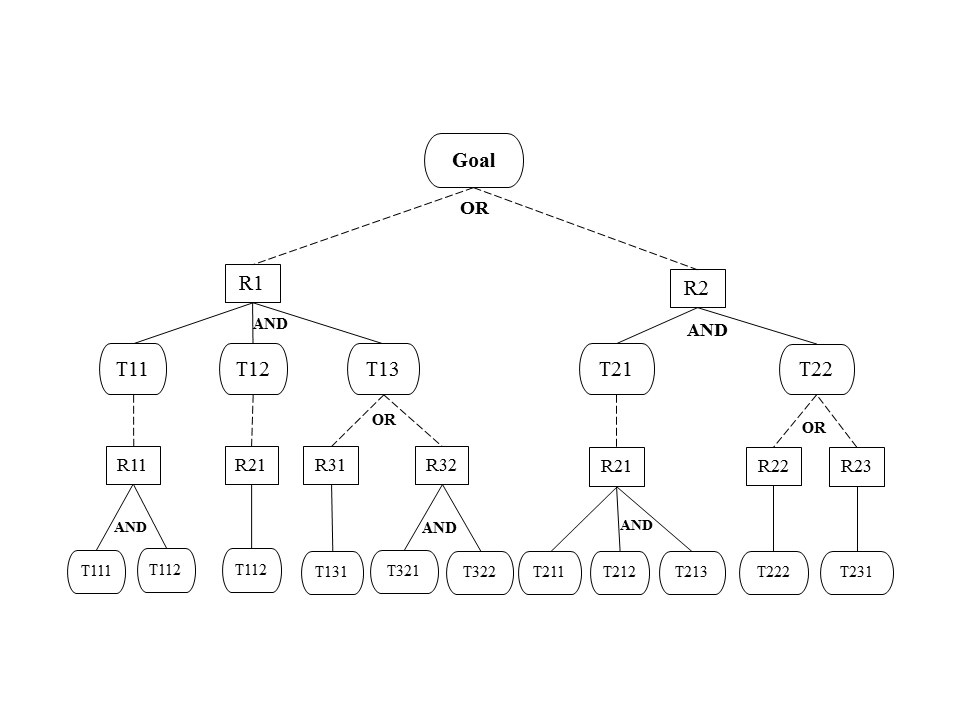
\includegraphics[width=\textwidth]{Pictures/htn1.png}
	\caption{\label{HTN tree representation} HTN tree representation}
\end{figure}


We denote two types of tasks; compound task or non-primitive task and primitive task or action. For example figure \ref{HTN example representation} represents a compound task Move (Obj, Room1, Room2, Door) which is decomposed into three primitive tasks $\{Pick-up (Obj), Walk (Room1, Room2, Door), Put-down(Obj)\}$.

\begin{figure}[h]
	\centering
	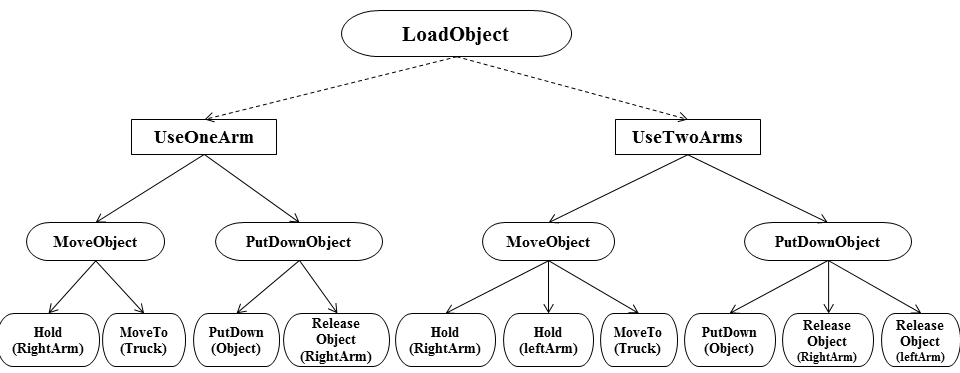
\includegraphics[width=\textwidth]{Pictures/example.png}
	\caption{\label{HTN example representation} HTN example representation}
\end{figure}


\subsubsection{HTN Recipe formalism}
An HTN recipe is used for decomposing compound tasks and has the form of a triple $\ R = (N, T, H)$ where $N$ is the name of the recipe which is unique such that no two recipes can have the same name. $T$ is a non-primitive task performed with this recipe and $H$ is a task network containing the set of subtasks of $T$, describing one way of performing the task T.


Using the HTN components formalism, we present now the domain knowledge and the HTN problem planning.

\par The Domain knowledge $D$ is a list of all the recipes in the HTN needed to decompose the HTN tasks. $\ D= [R1,. . . , Rn].$ Thus an HTN is a tree defined as a tuple $\ M =<T,D> $ where $T$ is the task network composed by all the tasks of the HTN and $D$ is the domain knowledge.

\par The planning problem $P$ is defined as a tree-tuple $\ P =< I, M, G>$ where $\ I$ is the initial state, $M$ is the domain problem defined by the HTN tree and $G$ is the goal task to achieve. $G$ belongs to the tasks of $M$ and the precondition of $G$ is true in $I$. The problem is to find a plan that solves $P$. HTN planning works by expanding tasks and resolving conflicts iteratively, until a conflict-free plan can be found that consists only of primitive tasks.

\par Planning proceeds using task decomposition that starts from the initial goal task $G$, expands this task using a corresponding recipe $R$, and breaks down the goal into sequence of simpler subtasks. This process is applied recursively until the planner reaches a sequence of fully ordered primitive tasks that can make a goal successful. Thus, the solution of the planning problem $P$ is a plan $\ \pi = [a1,.., an]$ is a sequence of primitive tasks $\ ai \in M$ , and $\ i \in [1,n].$

\par The HTN planners are becoming popular in different domains where several systems were developed these recent years such as SHOP \cite{nau1999shop}, SIPE \cite{wilkins1988practical} or NOAH \cite{sacerdoti1975structure}.

\par General purpose of planning as STRIPS and HTN relies on a complete model of the domain knowledge, that means if the model is not complete then, the planner won't be able to plan. This approach of planning is named \emph{Declarative representation}. Such representation of HTN requires a full modeling of HTN domain knowledge. Each
task in the HTN has at least one modeling specification that allows reasoning in planning. Despite the completeness of this representation, modeling such domain require significant knowledge-engineering effort if it is not impossible.

\section{Reactive HTNs}
Declarative approaches for planning attempt to predict the future. The planning is made in off-line phase that start from initial state to search for logical future states to reach a final goal state, using for that the modeling specifications in the domain knowledge. Once the plan is generated, the execution phase is launched in the environment.
\par In contrast with this approach, reactive HTNs propose an approach with no planning phase to predict the future states at all. Instead, they compute just the next task to perform in every instant. Moreover, because of the complexity of modeling a domain knowledge, reactive HTNs run through a hand-authored HTN with a procedural definition of the modeling specifications. Procedural definition of the domain knowledge means that the planner cannot reason about theses conditions, the conditions are script code (example JavaScript)  that can only be executed or evaluated in the current state.

\par The solution of a planning problem is to find a path through the HTN using recipe selection. Starting from the initial state and the goal task, The HTN incrementally generates a sequence of sub-goals by choosing recipes for decomposing tasks. The recipe is selected by the applicability condition at the state where this last can be evaluated. The modeling specifications are evaluated in the current state, if it returns the values true the HTN consider it as valid and continue the exploration of the HTN. However if the evaluation of any specification fails (returns false), the
HTN execution fails and we say that the HTN reaches a dead end. This situation is considered as hard failure. 

The execution is considered as complete if primitive tasks that make the goal successful are reached. Reactive HTN are becoming very popular in the field of controlling complex artificial intelligent systems exist performing in dynamic environment such as Dialog with the Disco system \cite{rich2009building} and RavenClaw \cite{bohus2003ravenclaw}.

\section{Plan execution, breakdown and recovery}
The declarative planners introduced before return a plan $\ \pi $ composed of a sequence of primitive tasks (actions), which is passed to the controller for the execution phase. The execution starts from the initial state and has to achieve the execution
of all the actions of the plan to reach the goal state. The execution of a STRIPS action is valid if its preconditions match subsets of the current observed world state immediately before the action is executed. The effects the executed action are added to the resulting state and the deleted effects are removed from it.

\par The HTN execution takes the STRIPS execution one step further by introducing the postcondition checks. As STRIPS primitive task (action) is applicable if its preconditions are valid in the current state of the world, in addition, the execution of the primitive task is considered as succeed only if its postconditions are part from the resulting state. Thus, the plan is a solution to a planning problem if it matches a subset of the current world state immediately after the last action in the plan is executed.

\par As the environment is dynamic, the controller monitors the environment at each execution step in order to prevent a breakdown. A breakdown occurs if any deviation from the steps defined in the constructed plan is detected, such deviation makes the executed plan invalid and the execution of plan stops. The breakdown
is identified if the world changes in an unexpected way that causes the execution failure of an action. The failure can be caused by one of these situations:
\begin{itemize}
	\item First, the action preconditions are no longer satisfied in the current state. For example, a robot that plans to walk from room1 to room2 through door1, arriving at door1 the wind blows and the door1 became close, this unexpected change invalidate the precondition of the action that is the door must be open.
	\item Second, the executed action leads to unexpected consequences, in this case the postconditions of the action are not satisfied.
\end{itemize}
%
\section{The problem}

Systems presented above need to plan, a complete definition of the domain knowledge which represent the real world faithfully. However,the dynamic definition of the environment in real problems implies unexpected changes that planner must predict and handle. For example, representing cooking problem such in Figure \ref{Cooking model example} involve representing all the actions and devices used. In addition, the model must contain tasks that can handle each change in the environment. For example, when modeling the cook task which involve heat the oven, if an electrical failure happens, then the planner has to react and restores electricity. However,  constructing such complete logical (declarative) model of real and complex problems that run in dynamic environment requires significant knowledge-engineering effort nearly impossible.  Thus, the domain knowledge is  incomplete which may lead the planner to face breakdowns. 
 \begin{figure}[h]
 	\centering
 	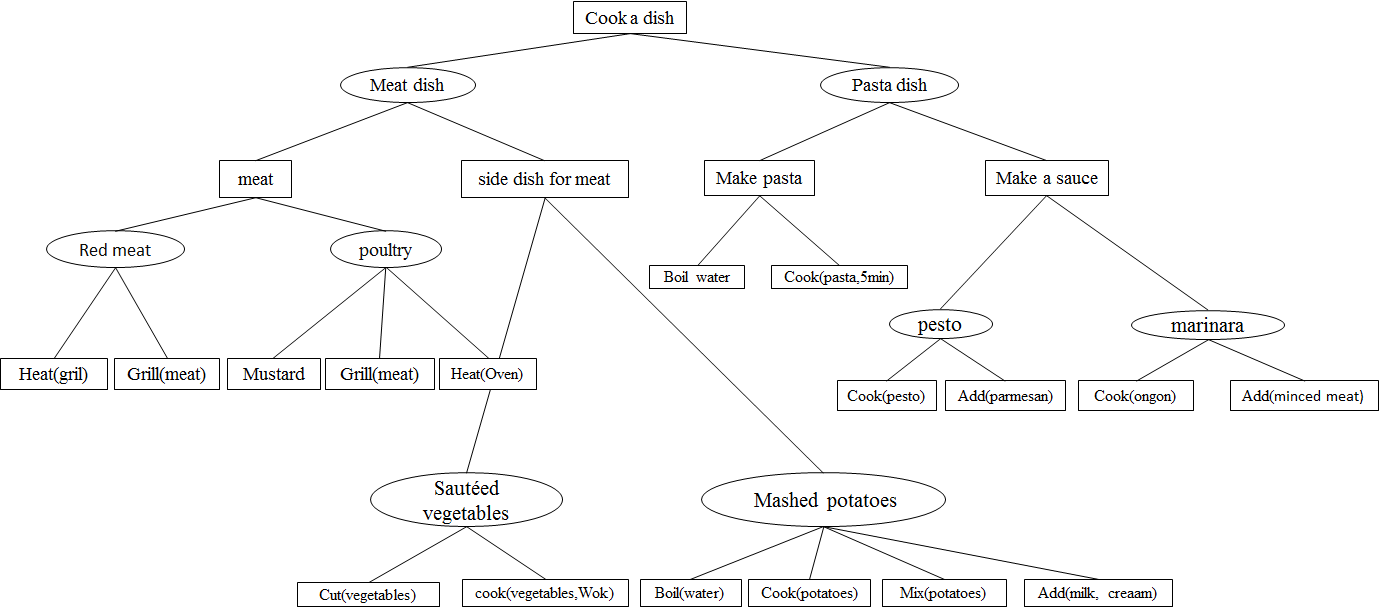
\includegraphics[width=\textwidth]{Pictures/cooking.png}
 	\caption{\label{Cooking model example} Cooking model example}
 \end{figure}
 

In addition, reactive HTNs take the position of using no planning process to detects the future state. Instead, the HTN plans only for the next task to be executed  based only on the current observable state. HTNs use procedural definition of the domain knowledge that can offer no reasoning and  uses an optimistic valuation of the conditions . This execution approach can lead the HTN to a state where no decomposition or execution are possible, this state is then called dead end. In such case, we say that the HTN executor faces a breakdown.Because of the procedural definition of the domain knowledge and the reactive formalism of the HTN, this later is unable to backtrack in order to find another way to achieve the goal task.
Therefore, the HTN can no longer continue its execution and the goal is impossible to achieve.

For example, lets the HTN describing the move\&paint task execution presented in Figure \ref{break example}. The HTN starts the decomposition from the top level goal and at each step it monitors the conditions of each task. Once it attempts primitive tasks, the execution in the real world starts. the HTN starts by executing the pickup(Object) task, by first evaluating its preconditions, after the execution of the task, the HTN evaluates its  postcondition. Arriving to the execution of the Walk task,  the world changes in unexpected way; assume that the wind blows and the door is now blocked.Thus, the preconditions of the Walk(room1, room2, door1) task (i.e IsOpen(Door)) are no longer valid. the HTN execution is then blocked and a breakdown is then detected.
 \begin{figure}[h]
 	\centering
 	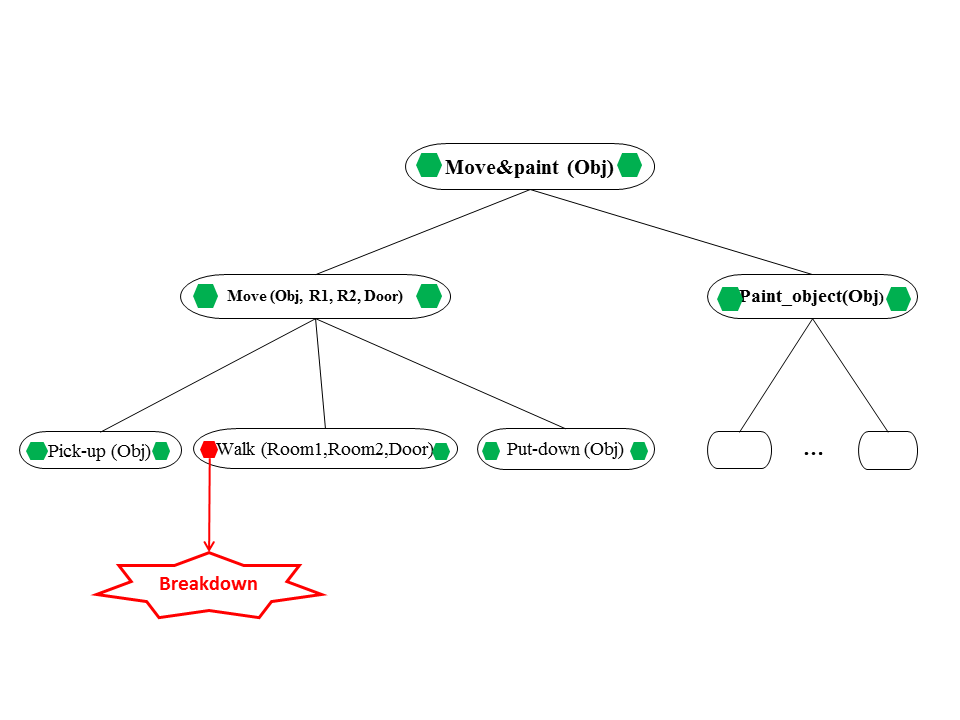
\includegraphics[width=\textwidth]{Pictures/break.png}
 	\caption{\label{break example} Breakdown situation in the move\&paint example}
 \end{figure}
 
 \section{Conclusion}
This chapter presented the background of our work.First, we presented and discussed the existing methods in the field of planning, from linear planning to hierarchical planning. Then we defined  the addressed problem which concerns breakdowns especially in reactive HTN, and the necessity of recovering from breakdowns taking in account the incompleteness of reactive HTN's knowledge domain.

In the next chapter (chapter3), we will put forward the existing approaches to recover from breakdowns and discuss their utility in the addressed problem. Next, we will present in chapter 4 the proposed solution to recover from breakdowns in reactive HTN with incomplete models and details the architecture of the plan recover system. 
 
%\chapter{Discolog approach} % Main chapter title

\label{Chapter 4} % For referencing the chapter elsewhere, use \ref{Chapter1} 

 In this Chapter, we introduce the Discolog system, a reactive HTN planning, execution, and plan-repairing system. Discolog is a   hybrid system that integrates  a reasoning engine modeled by STRIPS planner to a reactive HTN. We will first present an overview of the system, and next we will detail the system architecture.
\lhead{Chapter 4. \emph{Discolog approach}}

%In this section, we introduce our solution for plan recovery in reactive HTN. We also %present the description of the main procedures of plan recovery algorithm.


 Discolog uses reactive HTN style to achieve a goal with no prediction of future states at all.
 Starting from the top level goal, Discolog recursively decomposes tasks until it reaches a set of primitives tasks that can be directelly executed in the real world. 

 Nevertheless, because of procedural definition of reactive HTN domain knowledge which doesn't contain any logical information allowing the planner reasoning about task decomposition and execution, if the HTN faces breakdowns during the execution, it will be unable to backtrack  finding another decomposition that achieves the execution of the task.
 
 
In order to face this problem, Discolog uses a STRIPS planner to propose a plan recovery. It starts from the current observable state of the world and uses only the partial information available in the domain knowledge of the HTN to reason about. For that matter, Discolog extends the definition of certain HTN tasks in the domain knowledge from procedural definition to a declarative definition . An overview of the proposed execution and plan repair system is illustrated in Figure ~\ref{High level description of Discolog system}  .
		\begin{figure}[!h]
			\centering
			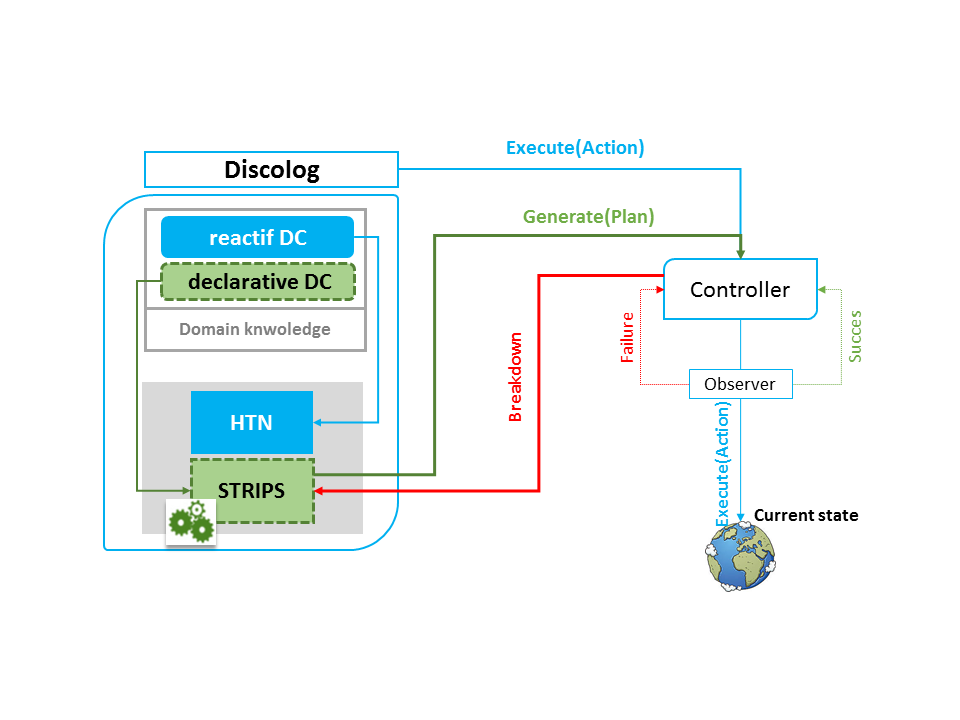
\includegraphics[width=250pt]{Pictures/architecture.png}
			\caption{\label{High level description of Discolog system} High level description of Discolog system}
		\end{figure}

The plan recovery in Discolog comprises two main procedures. The first one attempts to detect goal candidates to repair and the second invoke the STRIPS planner to propose a plan repair for these candidates. these procedures are described in the next sections.
\section{The Discolog algorithm}
Let \textit{HTN} be a model of an Hierarchical Task Network with a top level task \textit{Goal} to achieve, and Disco the the reactive HTN .To achieve \textit{Goal},  Disco  proceed as follow:
As showed in \ref{euclid}, Discolog starts from the top level goal \textit{Goal} and recursively decomposes tasks until it reaches a set of primitives tasks that can achieve \textit{Goal}.
Each task in Disco is defined with a \textit{status(Task)} $\in$ \{Live,Blocked,Done,Failed,Succeed\}.
\par Before decomposing a non primitive task or executing primitives task, Disco evaluate the precondition of the this task. If the current state holds the preconditions(Task) then status(Task) is updated to Live. otherwise, Status(Task)= not Live and the HTN execution is blocked.
The same, after the execution of a primitive task, Disco evaluate its postconditions. If postconditions(Task) are valid in the current state the status(Task) is updated to done or succeed, otherwise status(Task)= failed and the HTN execution become blocked.


At the end of the process, Disco(HTN,Goal) returns either Success(Goal is achieved) or failure if Disco faces breakdown. These breakdowns are detected if the top level goal is not achieved i.e Status(Goal) != Done and Disco has no decomposition or execution to propose. 

When such breakdown occurs, Discolog starts the recover procedure which will first look over the \textit{Goal} and its children to find task candidates which can be repaired from the current state in order to recover from the breakdown. The recover procedure is defined in the next sections.  
\begin{algorithm}
	\caption{DiscoLog algorithm }\label{euclid}
	\begin{algorithmic}[]
		\Procedure{Discolog}{HTN,Goal}
		\State $\textit{HTN} \gets\textit{ConstructModel()} $
		\State $\pi \gets Disco \textit{(HTN,Goal)}$
		\If {$ \pi \gets\textit{Success} $} 
		\State \Return $\textit{Success} $
		\Else 
		\State$ plan \gets Recover(Goal)$
		\If {(plan = \textit{null})}
		\State \Return Failure
		\Else 
		\For{$ \textbf{each}\text{ action }\textit{ai} \in plan $}
		\State  $\textit{Discolog} \text{(HTN,ai)}$
		\EndFor
		\EndIf
		\EndIf
		\\
		\EndProcedure \textbf{EndProcedure}
		\State 
		\Procedure{Recover}{Goal}
		\State $\textit{listCandidates}\gets\textit{findCandidate}{(G)} $
		\If {$ \textit{listCandidates = }\emptyset $} 
		\State \Return $\textit{null} $
		\Else 
		\State $\Pi \gets \emptyset$
		
		\For{$ \textbf{each} \textit{ candidate} \in \textit{listCandidates}$}
		\State $\Pi += InvokeSTRIPS(candidate,CurrentState)$
		\State  $Cost \gets \{ cost(\pi) | \pi \in  \Pi \} $
		\EndFor
		\EndIf
		\State \Return $\pi \in \Pi \text{ with minimum cost}(\pi)$
		\\
		\EndProcedure \textbf{EndProcedure}
		
		\State 
		\Procedure{FindCandidate}{Goal}
		\For{$ \textbf{each} \textit{ child} \in \textit{Goal}$}
		
		\If {$\text{(precondition(child)!=} \emptyset \text{ and}$
			\State$ \textbf{ status} (child)\notin\{\text{Done, Live, Blocked}\})$}
		\State $  \text{ add precondition(child) to candidates}$
		
		\ElsIf{$\text{(postcondition(child)!=}\emptyset 
			\text{ and } \textbf{ status} \text{(child)} \in \{\text{Failed}\}$}
		\State $\text{add postcondition(child) to candidates}$
		\EndIf
		\If {$(\textbf{status} \in \{\text{Live}\}\text{ and nonprimitive(child) and applicability(child)!=}\emptyset)$}
		\State add Applicabilitcondition(child) to candidates
		\EndIf
		\State $\textit{findCandidate} (children(child))$
		\EndFor
		\State \Return candidates
		\\
		\EndProcedure \textbf{EndProcedure}
		
	\end{algorithmic}
\end{algorithm}
\subsection{Goal candidates detection}
When a breakdown occurs, Discolog  will  first look over the goal task and its children to determine tasks in the HTN which are compromised by the breakdown, theses tasks are defined as task candidates for the plan recovery. 
For each task, we extract the condition failed because of the breakdown: 
\begin{itemize}
	\item	If the status of task is neither done nor live then the algorithm will attempts to repair its preconditions
	\item	If the status of task is failed then its postcondition are not valid and the repair algorithm will attempts to repair these postconditions.
	\item	if the task is nonprimitive and all its applicability conditions are invalid in the current state then the algorithm will attempts te replan to satisfy one of its applicability condition. 
\end{itemize}

Once, the list of candidate is identified, it is then passed to the InvokeStrips procedure.
As presented previously, a breakdown occur in a HTN if one of the task conditions fails, thus repairing a task using STRIPS planner is considered as repairing the failed condition of this task.
Once, the list of candidate is identified, the prolog STRIPS planner is called to propose a recovery plan.
\subsection{STRIPS repair planner}
In order to generate a plan, STRIPS has to constitute the planning problem to reason about. First  STRIPS constructs its domain knowledge by extracting partial information from the HTN domain knowledge and extends them to declarative definition. For that, Discolog convert all the primitive tasks to a declarative and logical formalism supported by STRIPS. Then for each candidate task, STRIPS takes as goal state  the failed task condition of the task candidate  and the current observable state is defined as the initial state.

Next, STRIPS tries to generate a linear plan to failed condition to reach a state where the failed condition is valid. Finally, Discolog calculate the best. i.e the  plan the plan with the minimum cost of execution and convert its actions to reactive formalism. this plan is then passed to Disco to be executed in the environment.

\section{Example}

Lets the HTN describing the move\&paint task execution presented in figure \ref{Plan recovery}. The HTN starts the decomposition from the top level goal and at each step it monitors the conditions of each task. Once it attempts primitive tasks, the execution in the real world starts. the HTN starts by executing the pickup(Object) by first evaluating its preconditions, after the execution of the task, the HTN evaluated the postconditions of the task. Arriving to the execution of the Walk task, , the world suddenly changes; assume that the wind blows and the door is now blocked thus the preconditions of the Walk(room1, room2, door1) task are no longer valid. Then a breakdown is detected and the recover procedure is called.


To recover from this breakdown, Discolog will first define the task candidates that can be repaired, which are the walk task with its preconditions and the move task with its postconditions. 

Once the list defined, it is passed to the STRIPS planner, which creates its domain knowledge as shown in figure \ref{Plan recovery}, next it generates a plan for both candidates. STRIPS returns the best plan that can repair the walk task composed. In this example the best plan consists of two primitives tasks; unlock(door) and open(door). 
This plan is converted to Disco tasks and executed. Once the plan recovery executed, Discolog continue the task decomposition from the current state to achieve the moveandpaint task. 

		\begin{figure}[h]
			\centering
			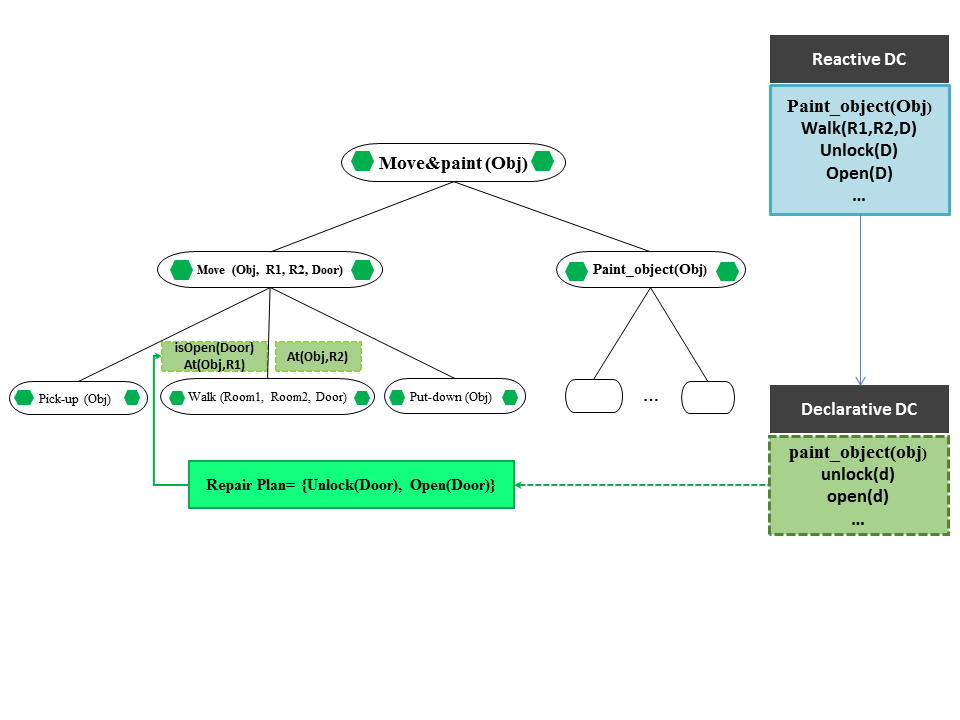
\includegraphics[width=.75\columnwidth]{Pictures/repair.png}
			\caption{\label{Plan recovery} Plan recovery for the move\&paint task using Discolog}
		\end{figure}
		
We present in this chapter the proposed solution and we detailed the conceptional procedure of this later. In the next chapter, we will present the implementation of the Discolog system.
%Let \textit{HTN} be a model of an Hierarchical Task Network with a top level task \textit{Goal} to achieve.To achieve \textit{Goal} Disco proceed as follow:
%
%
%Starting from the top level goal \textit{Goal}, Disco recursively decomposes tasks until it reaches a set of primitives tasks that can be directelly executed in the real world to achieve \textit{Goal}.
%Each task in Disco has a \textit{status(Task)} $\in$ \{Live,Blocked,Done,Failed,Succeed\}.
%\par Before decomposing a non primitive task or executing primitives task, Disco evaluate the precondition of the this task. If the current state holds the preconditions(Task) then status(Task) is updated to Live. otherwise, Status(Task)= Blocked and the HTN execution is blocked.
%The same, after the execution of a primitive task(execution of the grounding script), Disco evaluate its postconditions. If postconditions(Task) are valid in the current state the status(Task) is updated to done or succeed, otherwise status(Task)= failed and the HTN execution become blocked.
%\section{Description of the algorithm \ref{euclid}}
%
%
%At the end of the process, Disco(HTN,Goal) returns either Success(Goal is achieved) or failure if Disco faces breakdown. These breakdowns are detected if the top level goal is not achieved i.e Status(Goal) != Done and Disco has no decomposition or execution to propose. 
%
%When such breakdown occurs, the recovery algorithm will, first look over the \textit{Goal} and its children to find task candidates which can be repaired from the current state in order to recover from the breakdown. This process is handled by the procedure FindCandidates() described in the Algorithm \ref{euclid}.
% :
%\begin{itemize}
%	\item	If the status of task is neither done nor live then the algorithm will attempts to repair its preconditions
%	\item	If the status of task is failed then its postcondition are not valid and the repair algorithm will attempts to repair these postconditions.
%	\item	if the task is nonprimitive and all its applicability conditions are invalid in the current state then the algorithm will attempts te replan to satisfy one of its applicability condition. 
%\end{itemize}
%
%For example, the moveandpaint task which breakdowns in the execution of the walk task because its precondition "isOpen(door)" is no longer valid in the current state. 
%
%Once, the list of candidate is identified, the prolog STRIPS planner is called for each candidate and the solution with the shorter plan is returned to Disco to be executed in the real world.

 
%% Chapter 1

\chapter{Implementation} % Main chapter title

\label{Chapter 5} % For referencing the chapter elsewhere, use \ref{Chapter1} 

\lhead{Chapter 5. \emph{Implementation}} % This is for the header on each page - perhaps a shortened title
We described in previous chapters of this thesis, the  problem  being addressed and our proposition for a solution. In the following, we present the implementation of this solution. 

\section{Development environment }
In order to implement the hybrid system Discolog, we used the collaborative discourse engine Disco \cite{rich2009building} as reactive HTN to which we integrate a Prolog STRIPS planner  to support the plan repair process. 

The most important challenge within the realization of such hybrid system is to support heterogeneous formalisms of Disco and STRIPS. The system must be able to convert  the HTN domain knowledge from procedural formalism implemented in Java to a declarative one capable to run in Prolog  and  handle exceptions related to this conversion. 

For that purpose, we integrated to Disco the tuProlog \footnote{\url{http://apice.unibo.it/xwiki/bin/view/Tuprolog/}}  java-based light-weight Prolog engine to create a bridge that can use the logical Prolog planner from the Java procedural environment . the environment architecture is described  in figure \ref{implementation environment of Discolog}.
\begin{figure}[h]
	\centering
	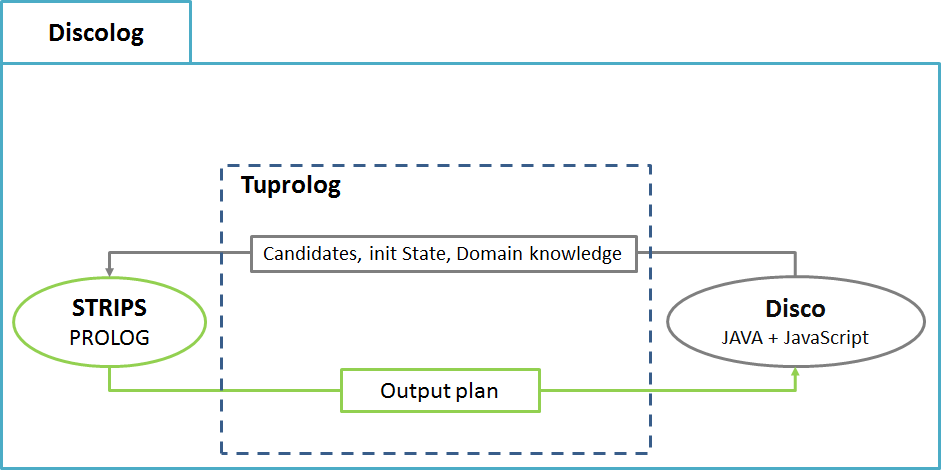
\includegraphics[width=\textwidth]{Pictures/archi1.png}
	\caption{\label{implementation environment of Discolog} implementation environment of Discolog}
\end{figure}


\section{Disco}
Disco \cite{rich2009building}is a collaborative discourse engine using reactive HTNS. The  most important feature of this reactive architecture is that allows the system to lead the user in a real time, without making any plan in advance. Disco's functional architecture is composed by a main component called \textit{task engine}. 
The function of the \textit{task engine}  is to load and validate a task model description and to maintain a representation of the current status of the user’s tasks.\cite{rich2009building}  


%----------------------------------------------------------------------------------------
\subsection{Disco task model}
Disco uses the ANSI/CEA-2018 standard for the procedural definition of the task model elements as described bellow :
\begin{itemize}
	\item \textit{Task}: The task model defines Task classes which are modeled using XML format, an example of the move\&paint implementation is showed in Appendix \ref{xml}. Primitive tasks may contain \textit{grounding script} parameter defined as JavaScript program which represent the effect of  the primitive task execution in the environment.
	
	\item \textit{Inputs and outputs} : Input includes all the data that may affect the execution of the task and output includes all data that can be affected by the execution of the task. these data type is defined in JavaScript.
	\item \textit{Conditions} : Task's conditions (Preconditions, postconditions ans applicability conditions) are defined as boolean JavaScript function to evaluate the execution of a task.

\end{itemize}

\section{Discolog implementation}
For the implementation of the Discolog system, we  faced some challenges. In addition to the management of heterogeneous environment, defining the level of information necessary to introduce in STRIPS domain knowledge required some reflection and designing a STRIPS planning algorithm able to provide effective solutions based on incomplete information in dynamic environment.
\subsection{The new Discolog API}
In order to implement the hybrid system Discolog we create an new  API divided in two mains folders :
	\begin{figure}[!h]
		\centering
		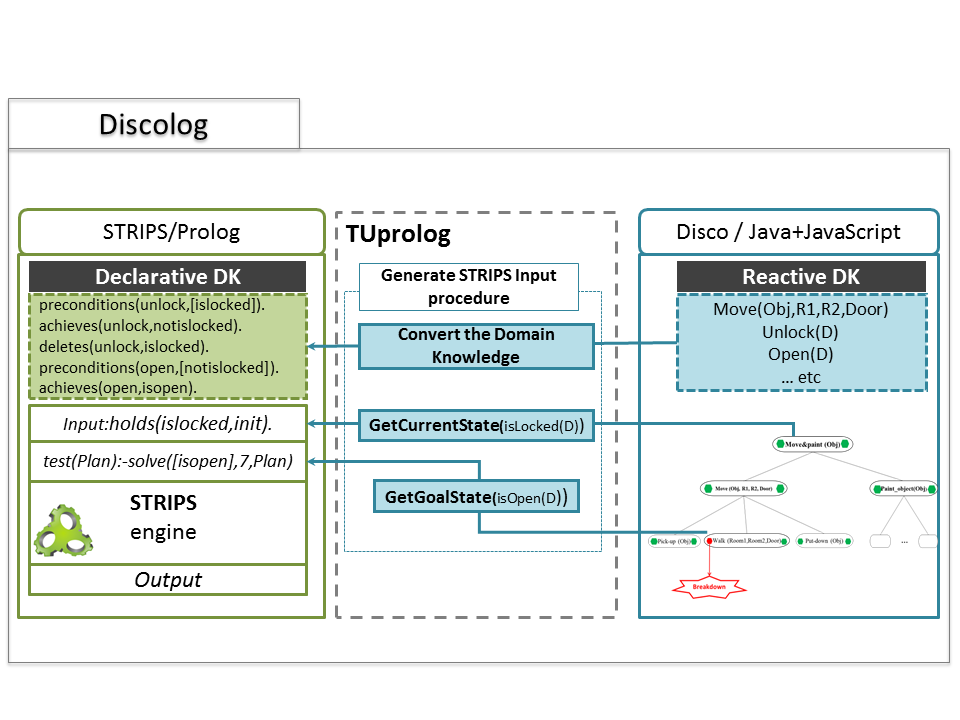
\includegraphics[width=\textwidth]{Pictures/input1.png}
		\caption{\label{input} Disco data generation in the moveandpaint example}
	\end{figure}
	
\subsubsection{ Disco extension }
We create an extension of Disco that can detect breakdowns and in such case, collects a candidates list for the plan recovery process. In addition, we manage to generate these candidates in the easiest way to be converted into Prolog formalism. The input Prolog planner is constituted in Disco via tuProlog as demonstrated in Figure \ref{input}.


 First, we start by creating the Prolog domain knowledge. Therefore, we extract all the primitives tasks and turn them to a Prolog formalism using tuProlog. Next, Disco observe the current state and convert it to the initial state. for example, in the move\&paint example, the current state where the breakdown occurs was IsLocked(Door) "the door is locked". Finally, the list of candidates is generated and each candidate is converted to a goal state to be achieve in Prolog.


\subsubsection{ Declarative Prolog implementation }
The main challenge faced in the creation of the STRIPS planner was to create an efficient means-end planning algorithm that can be integrated and executed  into tuProlog. Moreover, we had to define adequate structures that can receive the extracted domain knowledge. the STRIPS planner implemented is explained in Appendix \ref{AppendixB}.
% reference de STRIPS 


 Once STRIPS generate the plan recover, each action of this plan must be converted into primitive task formalism supported by Disco. Therefore we create a procedure that treat and convert the STRIPS plan output. An example of this procedure is shown  in Figure \ref{output} which describe how the plan repair is extracted for the move\&paint example. 

	\begin{figure}[!h]
		\centering
		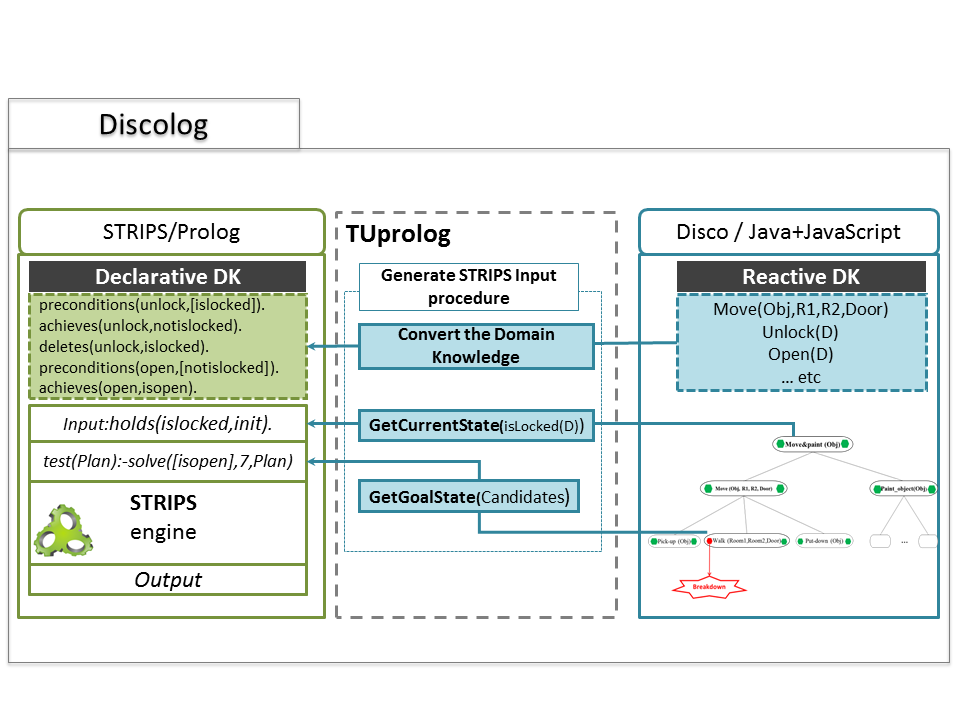
\includegraphics[width=\textwidth]{Pictures/output1.png}
		\caption{\label{output} Prolog data generation in the moveandpaint example}
	\end{figure}

\section{Conclusion}
In this chapter, we described the implementation of the Discolog system. First we introduce the environment of the implementation and we introduced the Disco system. Next we bring forward the new implemented Discolog API and explain each parts of this later.

In the next chapter, we present the experiments conducted to validate our system. 

%----------------------------------------------------------------------------------------


%\begin{multicols}{2}
%\lstinputlisting[language=XML]{Chapters/moveandpaint.xml}
%\end{multicols}
%\lstinputlisting[language=XML]{Chapters/moveandpaint.xml}
 

%----------------------------------------------------------------------------------------
%	THESIS CONTENT - APPENDICES
%----------------------------------------------------------------------------------------

\appendix % Cue to tell LaTeX that the following "chapters" are Appendices

% Include the appendices of the thesis as separate files from the Appendices folder
% Uncomment the lines as you write the Appendices

% Appendix A

\chapter{Move\&paint task in Disco} % Main appendix title

\label{xml} % For referencing this appendix elsewhere, use \ref{AppendixA}

\lhead{Appendix A. \emph{Move\&paint task in Disco}} % This is for the header on each page - perhaps a shortened title
\begin{verbatim}
<taskModel about="urn:limsi.fr:examples:moveandpaint
"xmlns="http://ce.org/cea-2018">

<task id="move_paint">
<input name="box" type="Box"/>
<subtasks id="movepaint">
<step name="move" task="move"/>
<step name="paint" task="paint"/>
<binding slot="$move.box" value="$this.box"/>
<binding slot="$move.from" value="$this.box.location"/>
<binding slot="$move.to" value="Room.ENUM.Painting_Room"/>
<binding slot="$paint.box" value="$move.new_box"/>
</subtasks>
</task>

<task id="move">
<input name="box" type="Box" modified="new_box"/>
<input name="from" type="Room"/>
<input name="to" type="Room"/>
<output name="new_box" type="Box"/>

<subtasks id="move_id">
<step name="pickup" task="pickup"/>
<step name="walk" task="walk"/>
<step name="putdown" task="putdown"/>
<binding slot="$pickup.box" value="$this.box"/>
<binding slot="$walk.box" value="$this.box"/>
<binding slot="$walk.from" value="$this.from"/>
<binding slot="$walk.to" value="$this.to"/>
<binding slot="$putdown.box" value="$walk.new_box"/>
<binding slot="$this.new_box" value="$walk.new_box"/>

</subtasks>
</task>

<task id="pickup">
<input name="box" type="Box"/>
</task>  

<task id="walk">
<input name="box" type="Box" modified ="new_box"/>
<input name="from" type="Room"/>
<input name="to" type="Room"/>
<output name="new_box" type="Box"/>

<precondition> isOpen() </precondition> 
<postcondition sufficient="true">
 $this.new_box.location == $this.to
 </postcondition> 
<script>$this.new_box.location = $this.to;</script>
</task>

<task id="putdown">
<input name="box" type="Box"/>
</task>

<task id="paint">
<input name="box" type="Box" modified ="new_box"/>
<output name="new_box" type="Box"/>
<precondition> 
$this.box.location == Room.ENUM.Painting_Room
 </precondition>
<postcondition sufficient="true"> $this.new_box.paint </postcondition>
<script> $this.new_box.paint = true; FIRST_PAINT = false; </script>
</task>

<task id="open">
<precondition> !isLocked(); </precondition>
<script> OPEN = true; </script>
</task>

<task id="unlock">
<script> LOCKED = false; </script>
</task>
<task id="recovery"/>  
<script init="true">

function Box (name,location, paint) {
this.name = name;
this.location = location;
this.paint = paint;
}

Box.prototype.toString = function () { 
return (this.name+ "[" + this.location+ "," + this.paint+"]");}

function Room (name) { 
this.name = name; 
}

Room.ENUM = { Room1 : new Room("room1"), 
Painting_Room : new Room("painting_room"),
 }
Room.prototype.toString = function ()
{ return this.name;}

var BOX1 = new Box("box1", Room.ENUM.Room1, false);
var OPEN = true;
var LOCKED = false;
var FIRST_PAINT = true;
var LOCATION = Room.ENUM.Room1; 
function isOpen() { return OPEN; }
function isLocked() { return LOCKED; }

</script>  
</taskModel>
\end{verbatim}
%\include{Appendices/AppendixB}
%\include{Appendices/AppendixC}

%----------------------------------------------------------------------------------------
%	BIBLIOGRAPHY
%----------------------------------------------------------------------------------------

\printbibliography[heading=bibintoc]

%----------------------------------------------------------------------------------------

\end{document}  
